\documentclass[11pt,fleqn]{report} 
\usepackage{mcs}

\usepackage[T1]{fontenc}
\usepackage{csquotes}
\usepackage{booktabs}
\usepackage{amssymb}
\usepackage{array}
\usepackage{enumitem}
\usepackage{tikz}
\usepackage{amsmath}
\usepackage{float}
\usepackage{longtable}
\usepackage{graphicx}

\usetikzlibrary{positioning}
\usetikzlibrary{arrows.meta}
\usetikzlibrary{shapes.geometric}

\hypersetup{
  pdftitle = {MSc thesis},
  pdfauthor = {Xiaoyan Xiong}
}

\coverauthor{Xiaoyan Xiong}
\supervisor{Le Viet Duc}
\covertitle{A Hierarchical Time-Aware Transformer for Flow-Level Network Intrusion Detection}
% A Hierarchical Time-Aware and Context-Aware Transformer for Flow-Level Network Intrusion Detection
% \doctype{Research Topics}
\doctype{Final Project}

%%%%%%%%%%%%%%%%%%%%%%%%%%%%%%%%%%%%%%%%%%%%%%%%%

\begin{document} 
\makecoverpage
\tableofcontents
% \setcounter{page}{1}  
\begin{abstract}      
  State the problem.
  Explain why the problem is a problem.
  Say something surprising.
  Describe consequences of your work

  % https://plg.uwaterloo.ca/~migod/research/beckOOPSLA.html
  
  \begin{keywords}    
   Machine leanring, Transformer, Time-aware, LSTM, GRU, CNN-LSTM, Representation
  \end{keywords}
\end{abstract}

%%%%%%%%%%%%%%%%%%%%%%%%%%%%%%%%%%%%%%%%%%%%%%%%%

\chapter{Introduction}

Modern computer networks generate large volumes of heterogeneous traffic across enterprise systems, cloud infrastructures, mobile networks, and Internet-of-Things (IoT) environments. Protecting such networks requires continuous monitoring and timely detection of malicious activities, including scanning, exploitation attempts, botnet communication, distributed denial-of-service (DDoS) attacks, and multi-stage intrusions. Network Intrusion Detection Systems (NIDSs) are therefore a fundamental component of cyber-security infrastructures \cite{Roesch1999,SommerPaxson2010}. However, building accurate and practical NIDSs remains challenging because modern attacks are increasingly distributed, adaptive, and temporally complex, while the widespread use of encryption limits direct payload inspection and shifts detection toward header, metadata, and behavioral traffic analysis \cite{Sharma2025EncryptedSurvey,Dong2025EncryptedPretrain}.

Signature-based systems such as Snort and Suricata are widely used in practice because they are interpretable, efficient, and effective against known threats \cite{Roesch1999,SuricataGuide2026}. These systems rely on manually designed rules to identify suspicious patterns in network traffic. Although rule-based detection remains valuable, it has inherent limitations: it depends on expert-maintained signatures, struggles with zero-day attacks and evolving variants, and may fail to capture attacks whose malicious behavior emerges only through temporal or contextual patterns across multiple flows \cite{SommerPaxson2010,Hozouri2025Survey}. As network traffic volume grows and attack behavior becomes more diverse, purely rule-based detection is insufficient as the sole detection mechanism.

Machine learning based NIDSs have been proposed to improve adaptability by learning decision boundaries from data rather than relying only on predefined rules. Classical approaches typically represent each flow using aggregated statistical features such as duration, packet counts, byte counts, packet rates, and inter-arrival-time statistics \cite{BuczakGuven2016,Ahmed2016Survey}. These flow-level features are compact and computationally efficient, making them attractive for large-scale detection. However, aggregation also removes important fine-grained information. In particular, packet ordering, burst patterns, direction changes, and irregular timing intervals may be lost when a complete flow is compressed into a single statistical vector. This loss is important because many attacks are not characterized only by total volume, but also by how packets evolve over time.

Deep learning approaches, including convolutional neural networks, recurrent neural networks, LSTMs, GRUs, and autoencoder-based models, have been explored to learn richer representations for intrusion detection \cite{Yin2017RNNIDS,Shone2018NNAE,Mirsky2018Kitsune}. These methods reduce the need for manual feature engineering and can model non-linear relationships in traffic data. Nevertheless, many existing deep learning NIDSs still operate primarily on flow-level aggregated inputs. Even when sequence models are used, they often model fixed-size flow feature sequences rather than the internal packet sequence of each flow. As a result, they only partially preserve the hierarchical structure of network traffic, where packets form flows and related flows form broader host-level or endpoint-level behaviors.

Transformer architectures provide a promising direction for this problem because self-attention can model long-range dependencies and process sequences efficiently in parallel \cite{Vaswani2017}. Recent Transformer-based NIDS studies have shown strong performance on network traffic classification and intrusion detection tasks \cite{Wu2022RTIDS,Han2023GTID,Manocchio2024FlowTransformer}. For example, time-aware Transformer designs demonstrate that temporal information can improve intrusion detection when traffic behavior depends on ordering and timing \cite{Han2023GTID}. FlowTransformer further shows the flexibility of Transformer-based architectures for flow-based NIDS evaluation \cite{Manocchio2024FlowTransformer}. However, many existing approaches still treat each flow as a flat representation and do not fully model the two-level structure of traffic: packet-level dynamics within a flow and contextual dependencies across flows.

This thesis addresses this gap by proposing a hierarchical two-stage framework for flow-level network intrusion detection. The starting point is raw PCAP traffic. A custom Suricata output plugin is used to extract two complementary views of the traffic: packet-level features and flow-level statistical features. Packet-level features preserve fine-grained temporal behavior, while flow-level statistical features summarize aggregate properties of each flow. After data cleaning and preprocessing, the first stage learns a flow representation using a time-aware packet-sequence Transformer. This Stage1 model processes packets within each flow as an ordered sequence and combines positional information with real-time temporal information. The learned packet-sequence representation is then fused with flow-level statistical features through a late-fusion mechanism to produce a final Stage1 embedding.

The second stage further models dependencies among flows. This is motivated by the observation that malicious behavior may not be fully visible from a single flow in isolation. For example, scanning, brute-force attempts, DDoS behavior, and multi-step intrusions often involve groups of related flows sharing temporal, source-host, destination-host, or endpoint-level context. Therefore, the Stage1 embeddings are used as inputs to a context-aware Stage2 Transformer. For each target flow, a context window is constructed using different strategies, including time-only context, source-host context, destination-host context, and endpoint-based context. The Stage2 model then learns whether the target flow is benign or malicious by considering both its own Stage1 representation and the behavior of related neighboring flows. This design is also related to recent work emphasizing cross-flow, graph-based, and contextual traffic modeling \cite{Deng2023FlowTopology,Zhong2024GNNSurvey,Li2024DoLLM}.

The central research problem of this thesis is therefore:

\begin{displayquote}
How can network intrusion detection benefit from packet-level temporal modeling and cross-flow contextual modeling while preserving the hierarchical structure of network traffic?
\end{displayquote}

To answer this question, the thesis studies two research questions:

\begin{itemize}
    \item \textbf{RQ1:} Does time-aware packet-sequence modeling produce more informative flow representations than flow-level aggregation alone?
    \item \textbf{RQ2:} Does incorporating cross-flow context improve flow-level intrusion detection compared with independent per-flow classification?
\end{itemize}

The main contributions of this thesis are as follows:

\begin{itemize}
    \item A PCAP-to-learning pipeline based on a custom Suricata plugin that extracts both packet-level and flow-level CSV features for flow-level intrusion detection.
    \item A Stage1 time-aware Transformer that models packet sequences within each flow using both positional and temporal information.
    \item A late-fusion design that combines learned packet-sequence embeddings with flow-level statistical features.
    \item A Stage2 context-aware Transformer that models relationships among neighboring flows using time-only, source-host, destination-host, and endpoint-based context construction strategies.
    \item A comprehensive empirical evaluation using F1, precision, recall, ROC-AUC, PR-AUC, confusion matrices, false positive rate, model parameters, training time.
    % , and inference time. 暂时去掉
\end{itemize}

Because intrusion detection datasets are often highly imbalanced, this thesis does not rely on accuracy alone. Instead, macro-F1 is used as the primary F1 measure because it gives equal importance to benign and attack classes. Macro-precision and macro-recall are reported to analyze the trade-off between false alarms and missed attacks. PR-AUC is emphasized because it is especially informative under class imbalance, while ROC-AUC measures threshold-independent ranking performance. Confusion matrices and false positive rate are also analyzed because, in operational NIDS settings, excessive false positives can overwhelm analysts and reduce the practical usability of a detector.

The remainder of this thesis is organized as follows. The next section reviews related work on rule-based NIDSs, classical machine learning, deep learning, Transformer-based traffic modeling, encrypted traffic analysis, and context-aware intrusion detection. The following sections describe the data extraction pipeline, preprocessing procedure, Stage1 time-aware Transformer, Stage2 context-aware Transformer, experimental setup, evaluation metrics, empirical results, discussion, and conclusion.

\chapter{Related Work}
\label{sec:related_work}

Network intrusion detection has evolved from manually specified signatures to data-driven models that learn representations from packet traces, flow records, or sequences of network events. The literature can be organized along two closely related dimensions: the granularity of the traffic representation and the scope of the modeled context. In terms of granularity, existing systems use
packet bytes, packet-header sequences, aggregated flow statistics, or learned flow embeddings. In terms of scope, most detectors classify each packet or flow independently, whereas a smaller body of work models temporal or relational dependencies among multiple flows. This section reviews these directions and positions the proposed hierarchical two-stage model with respect to them.

\section{Signature-Based and Statistical Flow-Based Detection}
\label{subsec:rw_signature_flow}

Signature-based NIDSs identify traffic patterns that match expert-defined rules. Snort established a lightweight and extensible architecture for real-time packet inspection \cite{Roesch1999}, while Suricata provides a modern multi-threaded engine and programmable logging facilities \cite{SuricataGuide2026}. These systems remain important in operational networks because their alerts are interpretable and their behavior is controllable. However, their effectiveness depends on the availability and maintenance of signatures, and previously unseen or behaviorally modified
attacks may not match known rules. More generally, Sommer and Paxson caution that learning-based NIDS research must account for the open-world character of network traffic and the semantic gap between laboratory benchmarks and operational deployment \cite{SommerPaxson2010}.

Classical machine-learning NIDSs commonly transform packets into bidirectional flow records and represent each flow by statistics such as duration, packet and byte counts, rates, TCP flags, and inter-arrival-time summaries. Surveys by Ahmed et al. and Buczak and Guven describe the broad use of decision trees, support-vector machines, nearest-neighbor methods, clustering, and ensemble
models for anomaly and intrusion detection \cite{Ahmed2016Survey,BuczakGuven2016}. Feature selection and hybrid classification can reduce dimensionality and improve conventional models
\cite{Aljawarneh2018}. The principal advantage of flow aggregation is efficiency: one fixed-dimensional vector represents a variable-length network conversation. Its principal limitation is information loss. Two flows with similar totals may exhibit different packet orders, direction changes, burst structures, or timing gaps. Consequently, a detector trained only on aggregate
statistics cannot directly learn the packet-level dynamics that generated those statistics.

The present work retains flow statistics because they provide a compact summary of volume and protocol behavior, but it does not treat them as a sufficient representation. Instead, they are used as a complementary modality and fused with an embedding learned from the packet sequence. This design also motivates the flow-statistics MLP baseline used to test whether packet-level temporal modeling contributes information beyond aggregation alone.

\section{Deep Learning for Packet and Flow Sequences}
\label{subsec:rw_deep_sequences}

Deep neural models reduce dependence on manually selected features by learning non-linear representations of network traffic. Recurrent NIDSs use hidden state to summarize ordered observations; for example, Yin et al. applied recurrent neural networks to intrusion detection and demonstrated their ability to learn sequential dependencies \cite{Yin2017RNNIDS}. Shone et al. combined a non-symmetric deep autoencoder with supervised classification to learn compact traffic representations \cite{Shone2018NNAE}. Kitsune instead used an ensemble of autoencoders for lightweight online anomaly detection, emphasizing the deployment value of compact and incrementally processed features \cite{Mirsky2018Kitsune}. Hybrid CNN--LSTM designs have also been used to combine local pattern extraction with recurrent temporal modeling \cite{Ullah2024IDSINT}.

Sequence construction is as important as the choice of neural architecture. Many studies apply an LSTM or GRU to a vector of flow features, where the ``sequence'' corresponds to feature dimensions rather than chronologically ordered packets or flows. Such a formulation can learn feature interactions but does not necessarily model network time. NetSentry addresses this issue more
directly by treating intrusion detection as a time-sensitive task and using ordered network observations to detect early-stage large-scale attacks \cite{LiuPatras2022NetSentry}. Its results support the broader argument that temporally correlated behavior can be more informative than independently classified records. Nevertheless, recurrence imposes sequential computation, and a single final hidden state may become a bottleneck for long or irregularly sampled sequences.

The Stage1 baselines in this thesis therefore include CNN, LSTM, GRU, BiLSTM, and time-augmented recurrent variants. These comparisons separate the value of the proposed traffic representation from the value of the Transformer architecture itself. In particular, they test whether explicit packet timing and attention-based aggregation improve minority-class detection relative to standard sequential encoders.

\section{Transformer-Based Traffic Representation}
\label{subsec:rw_transformers}

Transformers replace recurrent state transitions with self-attention, enabling each token to interact directly with all other tokens in a sequence and supporting parallel training \cite{Vaswani2017}. This mechanism is attractive for network traffic because attack evidence may be separated by many packets or flows. RTIDS demonstrated that a Transformer-based detector can provide robust intrusion classification on flow-oriented benchmarks \cite{Wu2022RTIDS}. Long et al. subsequently studied an encoder-based Transformer for cloud network intrusion detection
\cite{Long2024TransformerNIDS}, while IDS-INT combined Transformer-based transfer learning with imbalance handling and downstream neural components \cite{Ullah2024IDSINT}.

Two studies are especially close to the representation problem considered in Stage1. Han et al. proposed GTID, which combines packet- and session-level features with a time-aware Transformer; importantly, its temporal encoding uses inter-packet intervals rather than relying only on ordinal position \cite{Han2023GTID}. FlowTransformer provides a modular framework for examining input encodings, Transformer blocks, classification heads, model size, and runtime on flow-based NIDS datasets \cite{Manocchio2024FlowTransformer}. More recently, the memory flow Transformer was proposed to retain longer-term flow information and model complex relations in large sequential inputs \cite{Jiang2025MFT}. Collectively, these works establish that attention-based models can capture dependencies that are difficult to represent with a single aggregate vector. They also show that input encoding, pooling, sequence construction, and efficiency can matter as much as the nominal model family.

Despite this progress, three distinctions remain. First, positional order and elapsed network time are not equivalent: two adjacent packets may be separated by microseconds or seconds. Second, packet-sequence features and flow-level statistics describe complementary aspects of a connection and should be evaluated both separately and jointly. Third, a representation learned for one flow does not by itself explain whether that flow forms part of a distributed host-level pattern. The proposed Stage1 addresses the first two distinctions by combining positional and continuous-time encodings and by late-fusing the resulting packet-sequence embedding with flow statistics. Stage2 addresses the third by contextualizing the learned flow embeddings.

\section{Self-Supervised and Encrypted-Traffic Representation Learning}
\label{subsec:rw_ssl_encrypted}

The increasing use of encryption has shifted traffic analysis away from direct payload inspection toward packet sizes, directions, timing, header metadata, and learned representations. Recent surveys document this transition and the growing role of deep pre-training for encrypted traffic classification \cite{Sharma2025EncryptedSurvey,Dong2025EncryptedPretrain}. ET-BERT adapts bidirectional Transformer pre-training to contextualized datagram representations and demonstrates transfer to encrypted-traffic classification tasks \cite{Lin2022ETBERT}. Masked-autoencoder approaches similarly learn from unlabeled traffic by reconstructing hidden parts of an input representation \cite{Zhao2024MAETraffic,2024MAETraffic}. Contrastive learning provides another route to label-efficient NIDS by bringing related traffic views together while separating incompatible examples \cite{Li2024Contrastive}.

Other recent systems broaden the representation space. CoTNeT applies a contextual Transformer mechanism to encrypted-traffic features \cite{Huang2024CoTNet}, and DoLLM represents flow records in a form suitable for large-language-model-based DDoS detection \cite{Li2024DoLLM}. These approaches show that useful traffic representations can be learned without plaintext payloads and with reduced dependence on manually engineered signatures. However, encrypted-traffic classification and intrusion detection are not identical tasks: application identity may be stable even when attack behavior is sparse, evolving, or distributed across connections. The present thesis is therefore payload-independent but explicitly supervised for flow-level attack detection. Self-supervised pre-training is treated as a promising extension rather than a prerequisite of the proposed two-stage architecture.

\section{Temporal, Relational, and Cross-Flow Context}
\label{subsec:rw_cross_flow}

Most flow-based detectors assume that samples are conditionally independent. This simplification is convenient for batching and online inference, but it is often inconsistent with attack behavior. Scanning, password guessing, command and control, DDoS, and lateral movement can produce multiple individually ambiguous flows whose shared source, destination, endpoint, or temporal pattern is discriminative. Temporal models such as NetSentry demonstrate the value of ordered observations \cite{LiuPatras2022NetSentry}, while graph-based NIDSs make host and flow relations explicit. Deng et al. model flow topology with graph convolution for label-limited IoT intrusion detection \cite{Deng2023FlowTopology}; Xu et al. combine graph neural networks with self-supervised learning for network-flow intrusion detection \cite{Xu2024SSLGNN}. A recent survey by Zhong et al. organizes the rapidly growing use of graph neural networks in IDSs and highlights their ability to encode structural dependencies \cite{Zhong2024GNNSurvey}.

Graph methods provide expressive relational inductive bias, but constructing and updating a large communication graph can increase memory, latency, and deployment complexity. Window-based sequence models offer a complementary design point. A recent Transformer approach aggregates IoT flows into temporal windows and treats each flow as a token, allowing self-attention to capture inter-flow dependencies \cite{MartinReizabal2026FlowWindow}. The latest review of contextualized NetFlow NIDSs classifies context into temporal, relational, multimodal, and multi-resolution forms and emphasizes that evaluation must preserve causality and prevent cross-split context leakage \cite{ElMahdaouy2026ContextNetFlow}.

The Stage2 model in this thesis follows the window-based direction but differs in two respects. First, its tokens are not raw flow records; they are fused Stage1 embeddings that already encode packet-level temporal dynamics and flow statistics. Second, context membership is explicitly controlled through time-only, source-host, destination-host, and endpoint strategies. This enables a direct ablation of which relational assumption contributes useful evidence. The comparison with a no-context classifier tests whether gains originate from neighboring flows rather than from additional classifier capacity, while the LSTM, GRU, and CNN--LSTM Stage2 baselines test whether self-attention is needed to aggregate that context.

Table~\ref{tab:rw_model_comparison} summarizes the modeling scope of several representative Transformer-based approaches. The comparison is qualitative rather than performance-based because the studies use different datasets, labels, preprocessing pipelines, and evaluation protocols. Here, \emph{explicit elapsed time} means that timestamps or inter-arrival intervals are encoded directly; positional order or membership in a temporal window alone does not satisfy this criterion.

\begin{table}[t][H]
\centering
\caption{Qualitative comparison of representative Transformer-based traffic models. Entries describe the principal configuration reported in each cited study; extensible frameworks may support additional variants.}
\label{tab:rw_model_comparison}
\scriptsize
\setlength{\tabcolsep}{2pt}
\renewcommand{\arraystretch}{1.22}
\begin{tabular}{@{}p{1.85cm}p{2.65cm}p{1.55cm}p{2.15cm}p{2.45cm}p{1.85cm}p{1.85cm}@{}}
\toprule
\textbf{Method} &
\textbf{Primary input} &
\textbf{Intra-flow packet order} &
\textbf{Explicit elapsed time} &
\textbf{Inter-flow context} &
\textbf{Payload dependency} &
\textbf{Primary task} \\
\midrule
FlowTransformer \cite{Manocchio2024FlowTransformer} &
Flow records and statistics &
No &
Not explicitly encoded &
Yes; ordered flow sequence &
No &
Flow-level NIDS \\

GTID \cite{Han2023GTID} &
Packet headers and payload n-grams within a session &
Yes &
Yes; inter-packet intervals &
No &
Yes; payload n-grams &
NIDS \\

ET-BERT \cite{Lin2022ETBERT} &
Raw datagram bytes grouped into BURSTs &
Yes; byte and BURST order &
No; order only &
No cross-flow context &
Yes; encrypted bytes &
Encrypted-traffic classification \\

Flow-to-window Transformer \cite{MartinReizabal2026FlowWindow} &
Flow records in fixed-duration windows &
No &
Window-based order, not packet intervals &
Yes; temporal window &
No &
IoT NIDS and traffic classification \\

\textbf{Proposed} &
Packet-header sequence and flow statistics &
\textbf{Yes} &
\textbf{Yes; packet intervals} &
\textbf{Yes; time, source, destination, or endpoint} &
\textbf{No direct payload} &
\textbf{Flow-level NIDS} \\
\bottomrule
\end{tabular}
\end{table}

The table exposes the research gap without implying that the compared systems are directly rankable. FlowTransformer and the flow-to-window model capture relationships across flow records, but do not reconstruct the ordered packet dynamics inside each flow. GTID explicitly models packet order and inter-packet time, but operates on one session at a time and uses payload-derived n-grams. ET-BERT learns strong byte- and BURST-level representations from encrypted raw traffic, but its principal objective is encrypted-traffic classification rather than cross-flow intrusion detection. Among the representative systems in the table, the proposed framework is the only one that jointly combines payload-independent intra-flow packet modeling, explicit elapsed-time encoding, flow-statistical fusion, and configurable inter-flow context. This comparison therefore motivates the hierarchical separation between Stage1 and Stage2.
% \section{Datasets, Class Imbalance, and Evaluation Reliability}
% \label{subsec:rw_evaluation}

% Reported NIDS performance depends strongly on dataset construction and the
% evaluation protocol. Ring et al. distinguish packet- and flow-based datasets
% and identify recording environment, labeling, traffic diversity, and attack
% coverage as central dataset properties \cite{Ring2019Datasets}. More recent
% reviews show that the number of public NIDS datasets has grown substantially,
% but many datasets still contain limited realism, duplicated records, labeling
% errors, outdated attacks, or tool-dependent feature artifacts
% \cite{Goldschmidt2025Datasets,Pinto2025DatasetReview}. These problems can make
% random record-level splits overly optimistic when highly related flows, hosts,
% or capture periods occur in both training and test sets.

% Evaluation pitfalls are not limited to the data source. Arp et al. show that
% machine-learning security studies are vulnerable to leakage, inappropriate
% baselines, unrealistic assumptions, and metrics that obscure the actual
% security objective \cite{Arp2022DosDonts}. Class imbalance is particularly
% important in NIDS because high accuracy may coexist with poor attack recall.
% Focal loss is one possible training mechanism for emphasizing difficult and
% minority examples \cite{Lin2017FocalLoss}, but imbalance must also be reflected
% in reporting. Precision--recall analysis is generally more informative than
% ROC analysis when the positive class is rare
% \cite{SaitoRehmsmeier2015}. Accordingly, this thesis treats macro-F1 as the
% primary summary metric and reports macro-precision, macro-recall, attack-class
% precision/recall/F1, PR-AUC, ROC-AUC, the confusion matrix, and the false
% positive rate (FPR). Parameter count, training time, and inference time are also
% reported to expose the operational cost of contextual modeling.

% To reduce leakage risk, preprocessing parameters and decision thresholds should
% be selected without test-set access, and context windows should obey the chosen
% split policy. In particular, an online setting may use only information
% available before the target flow, whereas split-isolated evaluation must not
% allow validation or test flows to retrieve training-incompatible neighbors.
% These controls are essential for determining whether Stage2 learns transferable
% behavior or merely memorizes hosts, capture periods, or near-duplicate flows.

\section{Summary and Research Gap}
\label{subsec:rw_gap}

Prior research has established the usefulness of aggregate flow statistics,
deep sequential encoders, time-aware attention, self-supervised traffic
representations, and graph or window-based context. Nevertheless, these
directions are usually studied separately. Flow-statistical models are
efficient but discard packet dynamics; packet-sequence models usually classify
one flow at a time; and cross-flow models commonly operate on raw flow vectors
without first learning a timing-aware representation inside each flow.

This thesis addresses that gap with a hierarchical division of labor. Stage1
models packet order and elapsed time within each flow and late-fuses the learned
sequence representation with flow statistics. Stage2 then models dependencies
among the resulting flow embeddings under explicit temporal and endpoint-based
context policies. The design therefore connects two levels of network behavior:
\emph{intra-flow} packet dynamics and \emph{inter-flow} attack context. The
ablation studies are organized around the same distinction, allowing the work
to test separately whether time-aware packet modeling improves the flow
representation and whether cross-flow context improves the final detector.
% \section{Story Part}
% You can always cite books~\cite{Grune2012}, journal articles~\cite{Zoo2015} and conference publications~\cite{BabyCobol2020}.


% Preamble requirements:
% \usepackage{amsmath,amssymb,booktabs,array,enumitem,tikz}
% \usetikzlibrary{arrows.meta,positioning,shapes.geometric}


\chapter{Problem Formulation and System Overview}
\label{sec:problem_formulation}

This thesis formulates flow-level network intrusion detection as a hierarchical binary classification problem. The hierarchy arises from two nested structures in network traffic: packets form bidirectional flows, and related flows form larger temporal or host-level behaviors. Conventional flow-based classifiers typically compress the first structure into aggregate statistics and classify each resulting record independently. This is efficient, but it can discard
packet order and irregular timing and can overlook evidence distributed across several flows \cite{SommerPaxson2010,Han2023GTID,LiuPatras2022NetSentry}. Transformer-based NIDS research has demonstrated the value of both flow sequences and long-range dependencies \cite{Manocchio2024FlowTransformer,MartinReizabal2026FlowWindow}; however, the two levels of the hierarchy are not always modeled jointly. The objective of this work is therefore to learn a representation that first captures \emph{intra-flow} packet dynamics and then incorporates \emph{inter-flow} context for the final decision.

\section{Detection Setting and Design Requirements}
\label{subsec:detection_setting}

The detector operates on traffic extracted from PCAP traces. A custom Suricata
output plugin produces packet-level and flow-level records that can be aligned
through a flow identifier. Suricata is used as a practical traffic-processing
and logging engine \cite{Roesch1999,SuricataGuide2026}; its alert outcome is
used only during label construction. Alert counts, signature identifiers, rule
messages, and other direct indicators of the label are excluded from the model
input. The proposed detector also avoids direct payload content and instead
uses packet-header fields, packet direction and timing, aggregate flow
statistics, and metadata required to construct flow relationships. This setting
supports encrypted traffic because it does not require payload decryption.

The formulation is guided by the following requirements:

\begin{enumerate}[label=\textbf{R\arabic*:},leftmargin=*]
    \item \textbf{Hierarchical representation.} The model should preserve the
    packet sequence inside each flow and should also represent dependencies
    among related flows.

    \item \textbf{Explicit network time.} Packet position and elapsed time must
    be distinguishable. Adjacent packets can be separated by very different
    intervals, so ordinal position alone is insufficient
    \cite{Han2023GTID}.

    \item \textbf{Payload independence.} Predictions should not require raw
    application payloads, thereby reducing dependence on plaintext visibility
    and limiting exposure of content-sensitive data.

    \item \textbf{Causal context.} The context of a target flow may contain the
    target itself and eligible historical flows, but it must not contain future
    flows or labels. This requirement makes the formulation compatible with an
    online detector.

    \item \textbf{Imbalance-aware learning and evaluation.} Because malicious
    flows are the minority class, the learning objective and reported metrics
    must not be dominated by benign traffic.

    \item \textbf{Reproducible separation of data.} Preprocessing, context
    construction, model selection, and threshold selection must respect the
    training, validation, and test partitions. This limits common sources of
    experimental leakage in security machine learning
    \cite{Arp2022DosDonts,Ring2019Datasets}.
\end{enumerate}

The scope of the thesis is supervised binary flow classification rather than
attack prevention or rule generation. The output is a probability that the
target flow is malicious. Multiclass attack attribution, zero-day guarantees,
and automated response are outside the formal scope and are discussed as future
work.

\section{System Overview}
\label{subsec:system_overview}

Figure~\ref{fig:system_overview} summarizes the complete processing path. The
pipeline begins with raw PCAP traffic and ends with one prediction per target
flow. Packet and flow records are extracted together, aligned, cleaned, and
partitioned before model training. Stage1 transforms each packet sequence into
a time-aware representation and combines it with the corresponding statistical
flow representation through late fusion. The resulting Stage1 embedding is a
single fixed-dimensional vector per flow. Stage2 constructs a causal sequence
of these embeddings according to a selected context relation and predicts the
label of the target flow.

\begin{figure}[H]
\centering
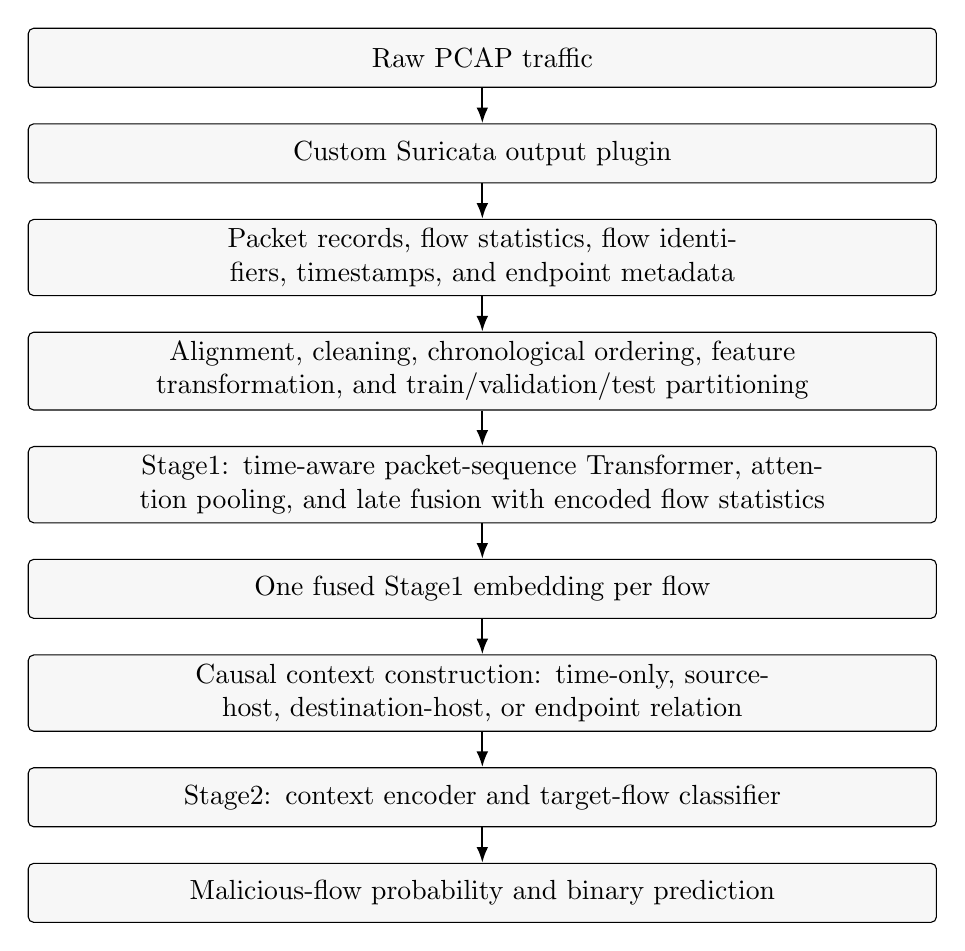
\begin{tikzpicture}[
    node distance=4.5mm,
    block/.style={
        rectangle,
        draw,
        rounded corners=2pt,
        align=center,
        text width=11.3cm,
        minimum height=7.5mm,
        fill=black!3
    },
    arrow/.style={-{Latex[length=2mm]},thick}
]
    \node[block] (pcap) {Raw PCAP traffic};
    \node[block, below=of pcap] (extract) {Custom Suricata output plugin};
    \node[block, below=of extract] (records) {Packet records, flow statistics, flow identifiers, timestamps, and endpoint metadata};
    \node[block, below=of records] (prep) {Alignment, cleaning, chronological ordering, feature transformation, and train/validation/test partitioning};
    \node[block, below=of prep] (stage1) {Stage1: time-aware packet-sequence Transformer, attention pooling, and late fusion with encoded flow statistics};
    \node[block, below=of stage1] (embedding) {One fused Stage1 embedding per flow};
    \node[block, below=of embedding] (context) {Causal context construction: time-only, source-host, destination-host, or endpoint relation};
    \node[block, below=of context] (stage2) {Stage2: context encoder and target-flow classifier};
    \node[block, below=of stage2] (output) {Malicious-flow probability and binary prediction};

    \draw[arrow] (pcap) -- (extract);
    \draw[arrow] (extract) -- (records);
    \draw[arrow] (records) -- (prep);
    \draw[arrow] (prep) -- (stage1);
    \draw[arrow] (stage1) -- (embedding);
    \draw[arrow] (embedding) -- (context);
    \draw[arrow] (context) -- (stage2);
    \draw[arrow] (stage2) -- (output);
\end{tikzpicture}
\caption{Overview of the proposed hierarchical two-stage intrusion-detection
pipeline.}
\label{fig:system_overview}
\end{figure}

% The two stages are trained sequentially in the current system. Stage1 is first
% optimized for flow-level classification and then used to export fused
% embeddings. Stage2 is trained on the exported embeddings and does not
% back-propagate gradients into Stage1. This separation permits independent
% evaluation of the representation learned in Stage1 and the contextual gain
% introduced by Stage2.

\section{Input Space and Notation}
\label{subsec:input_notation}

Let the dataset contain $N$ bidirectional flows sorted by flow start time. The
$i$th flow is represented by

\begin{equation}
\mathcal{F}_i =
\left(
    \mathbf{X}_i,
    \boldsymbol{\tau}_i,
    \mathbf{b}_i,
    \mathbf{s}_i,
    \mathbf{q}_i,
    y_i
\right),
\end{equation}

where the components are defined in
Table~\ref{tab:problem_notation}. The complete supervised dataset is

\begin{equation}
\mathcal{D}=\{\mathcal{F}_i\}_{i=1}^{N}.
\end{equation}

\begin{table}[H]
\centering
\caption{Notation used in the hierarchical problem formulation.}
\label{tab:problem_notation}
\small
\setlength{\tabcolsep}{5pt}
\renewcommand{\arraystretch}{1.15}
\begin{tabular}{@{}p{2.3cm}p{3.2cm}p{9.7cm}@{}}
\toprule
\textbf{Symbol} & \textbf{Domain} & \textbf{Meaning} \\
\midrule
$N$ & $\mathbb{N}$ & Number of flows. \\
$T_i$ & $\mathbb{N}$ & Number of observed packets in flow $i$ before sequence selection. \\
$L_{\max}$ & $\mathbb{N}$ & Maximum number of packet tokens retained for Stage1. \\
$\mathbf{X}_i$ & $\mathbb{R}^{L_i\times d_p}$ & Selected packet-feature sequence, where $L_i\leq L_{\max}$ and $d_p$ is the packet-feature dimension. \\
$\boldsymbol{\tau}_i$ & $\mathbb{R}^{L_i}$ & Packet timestamps or elapsed-time values aligned with $\mathbf{X}_i$. \\
$\mathbf{b}_i$ & $\{0,1\}^{L_{\max}}$ & Packet mask; one denotes an observed packet and zero denotes padding. \\
$\mathbf{s}_i$ & $\mathbb{R}^{d_f}$ & Flow-level statistical feature vector. \\
$\mathbf{q}_i$ & $\mathcal{Q}$ & Context metadata: source identifier, destination identifier, flow start time, and split membership. \\
$y_i$ & $\{0,1\}$ & Flow label, with zero for benign and one for malicious. \\
$\mathbf{z}^{(1)}_i$ & $\mathbb{R}^{d_1}$ & Fused Stage1 embedding for flow $i$. \\
$\mathcal{C}^{(r)}_i$ & Subset of $\{1,\ldots,i-1\}$ & Historical context indices for target flow $i$ under relation $r$. \\
$W$ & $\mathbb{N}$ & Maximum Stage2 sequence length, including the target flow when it is appended. \\
\bottomrule
\end{tabular}
\end{table}

Before padding, flow $i$ contains an ordered packet sequence

\begin{equation}
\mathcal{P}_i=
\left(p_{i,1},p_{i,2},\ldots,p_{i,T_i}\right),
\qquad
\tau_{i,1}\leq\tau_{i,2}\leq\cdots\leq\tau_{i,T_i}.
\end{equation}

Each retained packet is represented by a feature vector
$\mathbf{x}_{i,t}\in\mathbb{R}^{d_p}$. Packet timing can be expressed through
both elapsed time from the first retained packet and local inter-arrival time:

\begin{align}
e_{i,t} &= \tau_{i,t}-\tau_{i,1}, \\
\Delta\tau_{i,t} &=
\begin{cases}
0, & t=1,\\
\max(0,\tau_{i,t}-\tau_{i,t-1}), & t>1.
\end{cases}
\end{align}

A deterministic sequence-selection operator $\Pi_{L_{\max}}$ converts a
variable-length flow into at most $L_{\max}$ packet tokens:

\begin{equation}
\mathbf{X}_i=
\Pi_{L_{\max}}
\left(
    \mathbf{x}_{i,1},\ldots,\mathbf{x}_{i,T_i}
\right).
\end{equation}

The operator covers the evaluated head, head--tail, and random strategies. Its
choice changes which packets are retained but does not change the label or the
flow-level statistical vector. Padding is applied only after selection and is
excluded from attention and pooling through $\mathbf{b}_i$.

The context metadata can be written as

\begin{equation}
\mathbf{q}_i=(u_i,v_i,t_i^{0},\rho_i),
\end{equation}

where $u_i$ and $v_i$ are the source and destination identifiers, $t_i^{0}$ is
the flow start time, and $\rho_i\in\{\mathrm{train},\mathrm{val},\mathrm{test}\}$
denotes split membership. These identifiers determine context membership; they
are not labels and need not be directly embedded as numerical packet features.

\section{Stage1: Intra-Flow Representation Learning}
\label{subsec:stage1_formulation}

Stage1 learns one representation from the packets of a single flow. Packet
features are first projected into a $d_1$-dimensional latent space:

\begin{equation}
\mathbf{e}_{i,t}=W_p\mathbf{x}_{i,t}+\mathbf{c}_p.
\end{equation}

The model then adds information about ordinal position and network time:

\begin{equation}
\widetilde{\mathbf{e}}_{i,t}
=
\mathbf{e}_{i,t}
+\phi_{\mathrm{pos}}(t)
+\phi_{\mathrm{time}}(e_{i,t},\Delta\tau_{i,t}).
\end{equation}

The functions $\phi_{\mathrm{pos}}$ and $\phi_{\mathrm{time}}$ are written
separately because packet index and elapsed time convey different information.
The exact scaling, transformation, and fusion of the two encodings are specified
in the methodology chapter. A mask-aware Transformer encoder
\cite{Vaswani2017} produces contextualized packet states:

\begin{equation}
\mathbf{H}^{p}_i
=
\mathrm{Transformer}_{1}
\left(
    \widetilde{\mathbf{E}}_i;
    \mathbf{b}_i
\right),
\qquad
\mathbf{H}^{p}_i\in\mathbb{R}^{L_{\max}\times d_1}.
\end{equation}

The valid packet states are reduced to one packet-sequence representation by
attention pooling. For each valid position,

\begin{align}
r_{i,t} &=
\mathbf{w}_{a}^{\top}
\tanh(W_a\mathbf{h}^{p}_{i,t}+\mathbf{c}_a),\\
a_{i,t} &=
\frac{
    b_{i,t}\exp(r_{i,t})
}{
    \sum_{k=1}^{L_{\max}}b_{i,k}\exp(r_{i,k})
},\\
\mathbf{z}^{p}_i &=
\sum_{t=1}^{L_{\max}}a_{i,t}\mathbf{h}^{p}_{i,t}.
\end{align}

In parallel, the statistical flow vector is mapped into the same latent space:

\begin{equation}
\mathbf{z}^{f}_i=E_f(\mathbf{s}_i).
\end{equation}

Late fusion produces the final Stage1 embedding:

\begin{equation}
\mathbf{z}^{(1)}_i
=
\mathrm{Fuse}_{\psi}
\left(
    \mathbf{z}^{p}_i,
    \mathbf{z}^{f}_i
\right).
\label{eq:stage1_fusion}
\end{equation}

This formulation is deliberately different from repeating
$\mathbf{s}_i$ at every packet position. Packet-sequence learning is completed
before the aggregate statistics are fused, allowing the contribution of each
view to be measured independently. The Stage1 classifier is

\begin{equation}
\mathbf{p}^{(1)}_i
=
\mathrm{softmax}
\left(
    h_1(\mathbf{z}^{(1)}_i)
\right),
\end{equation}

where $p^{(1)}_{i,1}$ is the predicted probability of a malicious flow. This
prediction supports direct evaluation of Stage1 and therefore operationalizes
RQ1 before any cross-flow context is introduced.

\section{Stage2: Causal Inter-Flow Context Modeling}
\label{subsec:stage2_formulation}

After Stage1 inference, every flow has an embedding
$\mathbf{z}^{(1)}_i$. Let the complete set of strictly historical flows for
target $i$ be

\begin{equation}
\mathcal{H}_i=\{j\mid j<i\},
\end{equation}

where indices follow a stable chronological ordering. The system defines a
binary relation $R_r(i,j)$ for each context method $r$:

\begin{align}
R_{\mathrm{time}}(i,j)
&=1,\\
R_{\mathrm{src}}(i,j)
&=\mathbb{I}[u_i=u_j],\\
R_{\mathrm{dst}}(i,j)
&=\mathbb{I}[v_i=v_j],\\
R_{\mathrm{endpoint}}(i,j)
&=\mathbb{I}
\left[
    \{u_i,v_i\}\cap\{u_j,v_j\}\neq\varnothing
\right].
\end{align}

The eligible historical set is

\begin{equation}
\mathcal{A}^{(r)}_i
=
\left\{
    j\in\mathcal{H}_i
    \mid
    R_r(i,j)=1
\right\}.
\end{equation}

Given a maximum Stage2 length $W$, the context builder retains at most the
$W-1$ most recent eligible and deduplicated flows:

\begin{equation}
\mathcal{C}^{(r)}_i
=
\mathrm{Recent}_{W-1}
\left(
    \mathcal{A}^{(r)}_i
\right).
\label{eq:context_set}
\end{equation}

If
$\mathcal{C}^{(r)}_i=(j_1,\ldots,j_{K_i})$ with $K_i\leq W-1$, the Stage2 input
sequence is

\begin{equation}
\mathbf{Z}^{(r)}_i
=
\left[
    \mathbf{z}^{(1)}_{j_1},
    \ldots,
    \mathbf{z}^{(1)}_{j_{K_i}},
    \mathbf{z}^{(1)}_i
\right].
\label{eq:stage2_sequence}
\end{equation}

The current flow is appended as the final valid token. It does not reveal its
label; it provides the representation that Stage2 must classify. Padding and a
context mask are added when fewer than $W-1$ historical flows are available.
Because the histories are updated only after the current context is built,
Equations~\ref{eq:context_set}--\ref{eq:stage2_sequence} exclude both the future
and accidental self-duplication.

The primary formulation uses an online context policy: earlier flows can remain
available as state when the detector moves from training to validation and test
periods, but no label is retrieved and no future flow is visible. A
split-isolated policy can additionally restrict candidates to the target split
for sensitivity analysis. The policy used in each experiment must be reported
because context availability and the risk of leakage depend on it.

Stage2 projects and positionally encodes the context sequence before applying a
second sequence encoder:

\begin{equation}
\mathbf{G}^{(r)}_i
=
\mathrm{Transformer}_{2}
\left(
    \mathrm{Proj}_{2}(\mathbf{Z}^{(r)}_i)
    +\Phi_{2};
    \boldsymbol{\mu}_i
\right),
\end{equation}

where $\boldsymbol{\mu}_i$ is the context mask. Let
$\mathbf{g}^{(r)}_i$ denote the state at the final valid, target-flow position.
The context-aware probability is

\begin{equation}
\mathbf{p}^{(2,r)}_i
=
\mathrm{softmax}
\left(
    h_2(\mathbf{g}^{(r)}_i)
\right).
\label{eq:stage2_prediction}
\end{equation}

A no-context classifier provides the control condition

\begin{equation}
\mathbf{p}^{(\mathrm{nc})}_i
=
\mathrm{softmax}
\left(
    h_{\mathrm{nc}}(\mathbf{z}^{(1)}_i)
\right).
\end{equation}

Comparing Equation~\ref{eq:stage2_prediction} with the no-context control tests
whether neighboring flows add information beyond the capacity of another
classifier. Comparing the four relations tests which temporal or endpoint
assumption is most useful, thereby operationalizing RQ2.

\section{Learning Objectives and Decision Rule}
\label{subsec:learning_objectives}

Both stages solve an imbalanced binary classification problem. For stage
$\ell\in\{1,2\}$, let $p^{(\ell)}_{i,y_i}$ denote the probability assigned to
the correct class. The focal objective is

\begin{equation}
\mathcal{L}_{\ell}
=
-\frac{1}{|\mathcal{D}_{\mathrm{train}}|}
\sum_{i\in\mathcal{D}_{\mathrm{train}}}
\alpha^{(\ell)}_{y_i}
\left(
    1-p^{(\ell)}_{i,y_i}
\right)^{\gamma_{\ell}}
\log p^{(\ell)}_{i,y_i},
\label{eq:focal_objective}
\end{equation}

where $\gamma_{\ell}\geq0$ controls the emphasis on difficult examples and
$\alpha^{(\ell)}_{y_i}$ optionally controls class weighting
\cite{Lin2017FocalLoss}. Cross-entropy is recovered when
$\gamma_{\ell}=0$ and the class weights are uniform. The precise loss
configuration is treated as an experimental setting rather than an inherent
requirement of the architecture.

The current implementation uses sequential optimization. First,

\begin{equation}
\theta_1^{*}
=
\arg\min_{\theta_1}
\mathcal{L}_{1}(\theta_1),
\end{equation}

after which Stage1 exports
$\{\mathbf{z}^{(1)}_i(\theta_1^{*})\}_{i=1}^{N}$. Stage2 then solves

\begin{equation}
\theta_2^{*}
=
\arg\min_{\theta_2}
\mathcal{L}_{2}
\left(
    \theta_2;
    \{\mathbf{z}^{(1)}_i(\theta_1^{*})\}_{i=1}^{N}
\right).
\end{equation}

This formulation prevents Stage2 experiments from silently changing the
Stage1 representation and permits controlled comparisons among context methods
and Stage2 architectures.

For the malicious class, the final probability is
$p_i=p^{(2,r)}_{i,1}$, or $p_i=p^{(1)}_{i,1}$ when Stage1 is evaluated alone. A
binary decision is obtained using

\begin{equation}
\widehat{y}_i
=
\mathbb{I}[p_i\geq\delta^{*}],
\end{equation}

where the decision threshold is selected exclusively on the validation set:

\begin{equation}
\delta^{*}
=
\arg\max_{\delta\in\Delta}
M_{\mathrm{val}}(\delta).
\end{equation}

Here, $M_{\mathrm{val}}$ is the predefined threshold-selection metric and
$\Delta$ is the threshold search grid. The test set is evaluated once with the
selected model and threshold; it is not used to tune either quantity.

\section{Mapping the Formulation to the Research Questions}
\label{subsec:rq_mapping}

The formulation isolates the two contributions so that each research question
has a direct experimental test. Table~\ref{tab:rq_mapping} summarizes this
mapping.

\begin{table}[t]
\centering
\caption{Mapping between research questions, controlled comparisons, and
principal evidence.}
\label{tab:rq_mapping}
\small
\setlength{\tabcolsep}{5pt}
\renewcommand{\arraystretch}{1.15}
\begin{tabular}{@{}p{1.1cm}p{5.0cm}p{5.2cm}p{4.2cm}@{}}
\toprule
\textbf{RQ} & \textbf{Question in the formulation} & \textbf{Primary controlled comparisons} & \textbf{Principal evidence} \\
\midrule
RQ1 & Does $\mathbf{z}^{(1)}_i$ contain more useful attack information than aggregate flow statistics alone? & Flow-statistics MLP; LSTM/GRU baselines; positional/time encoding ablations; sequence-length and packet-selection studies; flow-fusion ablation. & Macro-F1, macro-precision, macro-recall, PR-AUC, ROC-AUC, confusion matrix, and FPR. \\
RQ2 & Does $\mathcal{C}^{(r)}_i$ improve prediction beyond an independent classifier on $\mathbf{z}^{(1)}_i$? & Stage1-only and no-context controls; time-only, source-host, destination-host, and endpoint context; window-size ablation; Transformer, LSTM, GRU, and CNN--LSTM Stage2 encoders. & The same detection metrics, together with context availability and changes in FP and FN. \\
% Cost & What computational cost is introduced by each representation and context model? & Stage1 and Stage2 models under the same implementation and hardware protocol. & Parameter count, training time, test inference time, and throughput where available. \\
\bottomrule
\end{tabular}
\end{table}

This separation is central to interpreting the final results. An improvement in
Stage1 supports the claim that packet timing and flow-statistical fusion improve
the representation of an individual flow. A further improvement from Stage2,
under the same Stage1 embeddings and test flows, supports the distinct claim
that related historical flows provide additional evidence. Efficiency results
then determine whether either improvement is operationally proportionate to its
computational cost.

\section{Chapter Summary}
\label{subsec:problem_summary}

The proposed problem is a causal, hierarchical, payload-independent
classification task. Stage1 maps an ordered and timed packet sequence together
with its flow statistics to a fused embedding. Stage2 constructs a bounded
historical context over these embeddings and predicts the label of the final
target flow. The separation between the stages supports controlled answers to
RQ1 and RQ2, while validation-only threshold selection, mask-aware sequence
processing, and explicit context policies establish the constraints required
for a reliable evaluation. The following chapters describe how the PCAP data
are transformed into the variables defined here and how the two model stages
are implemented and evaluated.

% Preamble requirements:
% \usepackage{amsmath,amssymb,booktabs,array,longtable,enumitem,tikz}
% \usetikzlibrary{arrows.meta,positioning,shapes.geometric}
%
% Bibliography files used by this section:
%   the proposal references.bib
%   doc/related_work_additions.bib
%   doc/dataset_preprocessing_additions.bib

\providecommand{\datasetfield}[1]{\texttt{\detokenize{#1}}}


\chapter{Dataset Construction and Preprocessing}
\label{sec:dataset_preprocessing}

This section describes how the proprietary packet capture was converted into
the two aligned data views required by the proposed hierarchical detector. The
description distinguishes among (i) fields retained in the raw CSV files,
(ii) predictors supplied to the Stage~1 model, and (iii) identifiers retained
only for constructing Stage~2 context. This distinction is important because a
field can be useful for record linkage without being an appropriate learning
feature. It also makes explicit which operations are fitted on training data
and which operations are deterministic transformations of the capture.
Careful documentation of provenance, labels, transformations, and partitions
is essential for credible NIDS evaluation
\cite{Shiravi2012DatasetGeneration,Ring2019Datasets,Goldschmidt2025Datasets,
Pinto2025DatasetReview}.

\section{Data Provenance and Scope}
\label{subsec:data_provenance}

The experiments use the packet capture
\datasetfield{ar002_et12_20260511_001.pcap}, whose file size is approximately
$8.62\,\mathrm{GB}$. The trace was supplied by a company colleague after being
downloaded from the company network with an organizational traffic-collection
tool. The thesis author therefore starts from an already acquired PCAP rather
than generating traffic in a laboratory testbed. Unlike CICIDS-style datasets,
in which benign profiles and attacks are deliberately executed under a
controlled schedule \cite{Sharafaldin2018CICIDS}, this capture represents
naturally occurring enterprise traffic as observed by the collection point.
It may consequently provide greater environmental realism, but its traffic
mix, host population, visibility, and attack coverage are specific to one
organization and one capture period.

The dataset is proprietary and is not presented as a public benchmark. The raw
PCAP and CSV files contain network identifiers, including IP addresses and
ports, that can be sensitive. Accordingly, this thesis reports only aggregate
statistics and does not print individual addresses. Any artifact released
outside the authorized environment should replace host identifiers with
consistent pseudonyms, remove unnecessary endpoint fields, and be reviewed
against the company's data-governance policy. Consistent pseudonyms are
preferable to deleting all identifiers because Stage~2 requires equality tests
between host identifiers; the mapping itself need not be released. The current
extraction code retains raw addresses in local metadata, so pseudonymization is
a release requirement rather than a claimed property of the present CSV files.

\section{PCAP-to-CSV Extraction}
\label{subsec:pcap_extraction}

The PCAP is replayed through Suricata, an open-source network threat detection
engine \cite{Roesch1999,SuricataGuide2026}. A custom C output plugin located at
\datasetfield{suricata-plugin/custom-out.c} registers both a packet logger and
a flow logger. Suricata exposes low-level packet and flow logging interfaces to
custom output modules; the plugin uses these interfaces to emit two CSV files
in one processing pass. This design avoids reconstructing packet-to-flow
membership in a separate tool and preserves a shared bidirectional
\datasetfield{flow_id} across both views.

Figure~\ref{fig:data_construction_pipeline} summarizes the data-construction
path. Packet rows preserve within-flow order and microsecond timestamps, while
the flow logger maintains online aggregates and writes one statistical record
per completed flow. The flow schema follows the broad feature families used by
CICFlowMeter/CICIDS-style data, while adding explicit indicators for whether
the initial forward and backward TCP window values are available
\cite{Sharafaldin2018CICIDS}.

\begin{figure}[H]
    \centering
    \begin{tikzpicture}[
        node distance=7mm and 8mm,
        block/.style={draw, rectangle, rounded corners=2pt, align=center,
                      minimum height=9mm, text width=29mm, font=\small},
        smallblock/.style={draw, rectangle, rounded corners=2pt, align=center,
                           minimum height=9mm, text width=27mm, font=\small},
        arrow/.style={-{Latex[length=2mm]}, thick}
    ]
        \node[block] (pcap) {Enterprise PCAP\\$8.62\,\mathrm{GB}$};
        \node[block, right=of pcap] (suricata) {Suricata + custom\\output plugin};
        \node[smallblock, above right=5mm and 9mm of suricata] (packet) {Packet CSV\\$11{,}750{,}727\times40$};
        \node[smallblock, below right=5mm and 9mm of suricata] (flow) {Flow CSV\\$421{,}898\times77$};
        \node[block, right=9mm of packet] (align) {Integrity checks and\\\datasetfield{flow_id} alignment};
        \node[block, below=of align] (split) {Chronological\\flow-level split};
        \node[block, below=of split] (tensor) {Train-fitted transforms\\and model tensors};

        \draw[arrow] (pcap) -- (suricata);
        \draw[arrow] (suricata) -- (packet);
        \draw[arrow] (suricata) -- (flow);
        \draw[arrow] (packet) -- (align);
        \draw[arrow] (flow) -- (align);
        \draw[arrow] (align) -- (split);
        \draw[arrow] (split) -- (tensor);
    \end{tikzpicture}
    \caption{Construction and preprocessing path from the proprietary PCAP to
    Stage~1 tensors and Stage~2 metadata.}
    \label{fig:data_construction_pipeline}
\end{figure}

No raw application payload bytes are supplied to either learning stage. The
packet table does contain \datasetfield{payload_len}, which is a scalar length
derived from packet metadata, but it does not contain payload content. This
wording is deliberate: the detector is payload-content independent, not
entirely free of payload-related metadata. Alert signatures, rule identifiers,
alert messages, and alert counts are also excluded from the predictors.

\section{Alert-Derived Label Construction}
\label{subsec:label_construction}

The custom logger derives binary labels from Suricata's alert state. Let
$a(p_i)$ denote the number of Suricata alerts attached to packet $p_i$. The
packet label is
\begin{equation}
    y_i^{\mathrm{pkt}}
    = \mathbb{I}\!\left[a(p_i)>0\right],
    \label{eq:packet_alert_label}
\end{equation}
where $\mathbb{I}[\cdot]$ is the indicator function. A flow is labelled
positive when at least one of its packets triggers an alert:
\begin{equation}
    y_f
    = \max_{p_i\in\mathcal{P}_f} y_i^{\mathrm{pkt}},
    \label{eq:flow_alert_label}
\end{equation}
where $\mathcal{P}_f$ is the set of packets assigned to flow $f$. Thus,
\datasetfield{packet_label}=1 indicates an alert-triggering packet and
\datasetfield{label}=1 indicates an alert-associated flow.

These are programmatic or \emph{weak} labels rather than independent expert
ground truth \cite{Ratner2017Snorkel}. In particular, label~0 means that the
configured Suricata rules did not generate an alert; it does not prove that the
traffic is benign. Conversely, a positive label inherits any false positives
of the deployed ruleset. The experiments therefore measure how well the model
learns and contextualizes Suricata-alert-associated behavior, rather than
establishing guaranteed detection of every intrusion or zero-day attack.
Potential label errors can affect both training and test estimates, and this
limitation must be retained when interpreting the results
\cite{Northcutt2021ConfidentLearning}.

% To prevent direct target leakage, neither \datasetfield{packet_label} nor
% \datasetfield{label} is included in a feature vector. Suricata alert metadata
% is likewise absent from the model input. For reproducibility, the final
% experiment manifest should record the Suricata version, rule-set name and
% version, rule update date, command-line/configuration checksum, custom-plugin
% commit, and PCAP checksum. These items determine the weak-labeling function and
% cannot be reconstructed from the CSV dimensions alone.

\section{Raw Dataset Composition}
\label{subsec:raw_composition}

The extraction produced the two aligned tables summarized in
Table~\ref{tab:raw_dataset_summary}. The packet table contains
$11{,}750{,}727$ rows and 40 columns; the flow table contains $421{,}898$ rows
and 77 columns. Dividing the two row counts gives an average of approximately
$27.85$ logged packets per flow before sequence truncation. This average does
not imply that flow lengths are uniform; network packet counts are typically
heavy-tailed, which motivates an explicit maximum sequence length.

\begin{table}[H]
    \centering
    \caption{Raw extracted dataset summary.}
    \label{tab:raw_dataset_summary}
    \begin{tabular}{@{}lrrp{5.7cm}@{}}
        \toprule
        Data view & Rows & Columns & Primary role \\
        \midrule
        Packet CSV & 11,750,727 & 40 & Ordered packet-header, protocol,
        direction, and inter-arrival observations within flows \\
        Flow CSV & 421,898 & 77 & One flow-level target, aggregate
        statistics, and context-construction metadata per flow \\
        \bottomrule
    \end{tabular}
\end{table}

The binary flow-label distribution is shown in
Table~\ref{tab:flow_label_distribution}. Of the $421{,}898$ flow records,
$405{,}254$ are labelled 0 and $16{,}644$ are labelled 1. The positive
prevalence and imbalance ratio are therefore
\begin{align}
    \pi_1 &= \frac{16{,}644}{421{,}898} = 0.03945
             \quad (3.945\%), \\
    \mathrm{IR} &= \frac{405{,}254}{16{,}644} = 24.35:1.
    \label{eq:dataset_imbalance}
\end{align}

\begin{table}[H]
    \centering
    \caption{Flow-level alert-derived label distribution.}
    \label{tab:flow_label_distribution}
    \begin{tabular}{@{}llrr@{}}
        \toprule
        Label & Interpretation & Count & Proportion \\
        \midrule
        0 & No Suricata alert observed in the flow & 405,254 & 96.055\% \\
        1 & At least one alert-triggering packet & 16,644 & 3.945\% \\
        \midrule
        Total & & 421,898 & 100.000\% \\
        \bottomrule
    \end{tabular}
\end{table}

An always-negative classifier would consequently obtain approximately
$96.055\%$ accuracy while detecting no positive flows. Accuracy and weighted
averages are therefore secondary metrics for this dataset. The evaluation
focuses on macro-precision, macro-recall, macro-F1, ROC-AUC, PR-AUC, the
confusion matrix, and the false-positive rate. PR-AUC is particularly useful
when the positive class is rare \cite{SaitoRehmsmeier2015}. The large benign
population also makes the false-positive rate operationally important: a small
percentage of $405{,}254$ negative flows can still produce a substantial alert
volume.

\section{Raw Packet and Flow Schemas}
\label{subsec:raw_schemas}

Tables~\ref{tab:packet_schema} and~\ref{tab:flow_schema} group all raw columns
by function. The grouping is descriptive; it does not imply that every raw
column is used as a predictor.

\begin{longtable}{@{}>{\raggedright\arraybackslash}p{0.20\textwidth}
                         >{\raggedright\arraybackslash}p{0.75\textwidth}@{}}
    \caption{Complete packet CSV schema grouped by function.}
    \label{tab:packet_schema} \\
    \toprule
    Group & Raw columns \\
    \midrule
    \endfirsthead
    \multicolumn{2}{c}{\tablename\ \thetable\ -- continued from previous page} \\
    \toprule
    Group & Raw columns \\
    \midrule
    \endhead
    \midrule
    \multicolumn{2}{r}{Continued on next page} \\
    \endfoot
    \bottomrule
    \endlastfoot
    Record identity and time &
    \datasetfield{record_type}, \datasetfield{packet_id},
    \datasetfield{timestamp_us}, \datasetfield{ts_sec},
    \datasetfield{ts_usec}, \datasetfield{flow_id} \\
    Endpoints and protocol &
    \datasetfield{direction}, \datasetfield{ip_version},
    \datasetfield{src_ip}, \datasetfield{dst_ip},
    \datasetfield{src_port}, \datasetfield{dst_port},
    \datasetfield{protocol}, \datasetfield{l7_proto} \\
    Length and header metadata &
    \datasetfield{pkt_len}, \datasetfield{ip_len},
    \datasetfield{payload_len}, \datasetfield{ttl_or_hop_limit},
    \datasetfield{tcp_window}, \datasetfield{tcp_header_len},
    \datasetfield{udp_len} \\
    Transport indicators &
    \datasetfield{has_tcp}, \datasetfield{has_udp},
    \datasetfield{has_icmp} \\
    TCP state and flags &
    \datasetfield{tcp_seq}, \datasetfield{tcp_ack},
    \datasetfield{tcp_flags}, \datasetfield{tcp_fin},
    \datasetfield{tcp_syn}, \datasetfield{tcp_rst},
    \datasetfield{tcp_psh}, \datasetfield{tcp_ack_flag},
    \datasetfield{tcp_urg}, \datasetfield{tcp_ece},
    \datasetfield{tcp_cwr} \\
    ICMP metadata &
    \datasetfield{icmp_type}, \datasetfield{icmp_code} \\
    Inter-arrival time &
    \datasetfield{flow_iat_us}, \datasetfield{direction_iat_us} \\
    Target &
    \datasetfield{packet_label} \\
\end{longtable}

The two packet timing fields have different semantics.
\datasetfield{flow_iat_us} is the elapsed time from the previous packet in the
same bidirectional flow, whereas \datasetfield{direction_iat_us} is measured
from the previous packet in the same direction. Both use microseconds and are
zero for the first applicable observation.

\begin{longtable}{@{}>{\raggedright\arraybackslash}p{0.20\textwidth}
                         >{\raggedright\arraybackslash}p{0.75\textwidth}@{}}
    \caption{Complete flow CSV schema grouped by function.}
    \label{tab:flow_schema} \\
    \toprule
    Group & Raw columns \\
    \midrule
    \endfirsthead
    \multicolumn{2}{c}{\tablename\ \thetable\ -- continued from previous page} \\
    \toprule
    Group & Raw columns \\
    \midrule
    \endhead
    \midrule
    \multicolumn{2}{r}{Continued on next page} \\
    \endfoot
    \bottomrule
    \endlastfoot
    Identity and time &
    \datasetfield{flow_id}, \datasetfield{flow_start_timestamp_us},
    \datasetfield{flow_end_timestamp_us} \\
    Endpoints and protocol &
    \datasetfield{source_ip}, \datasetfield{source_port},
    \datasetfield{destination_ip}, \datasetfield{destination_port},
    \datasetfield{protocol} \\
    Directional volume &
    \datasetfield{total_fwd_packets}, \datasetfield{total_backward_packets},
    \datasetfield{total_length_of_fwd_packets},
    \datasetfield{total_length_of_bwd_packets} \\
    Directional length statistics &
    \datasetfield{fwd_packet_length_max},
    \datasetfield{fwd_packet_length_min},
    \datasetfield{fwd_packet_length_mean},
    \datasetfield{fwd_packet_length_std},
    \datasetfield{bwd_packet_length_max},
    \datasetfield{bwd_packet_length_min},
    \datasetfield{bwd_packet_length_mean},
    \datasetfield{bwd_packet_length_std} \\
    Overall rate and timing &
    \datasetfield{flow_duration}, \datasetfield{flow_bytes_per_s},
    \datasetfield{flow_packets_per_s}, \datasetfield{flow_iat_mean},
    \datasetfield{flow_iat_std}, \datasetfield{flow_iat_max},
    \datasetfield{flow_iat_min} \\
    Directional inter-arrival time &
    \datasetfield{fwd_iat_total}, \datasetfield{fwd_iat_mean},
    \datasetfield{fwd_iat_std}, \datasetfield{fwd_iat_max},
    \datasetfield{fwd_iat_min}, \datasetfield{bwd_iat_total},
    \datasetfield{bwd_iat_mean}, \datasetfield{bwd_iat_std},
    \datasetfield{bwd_iat_max}, \datasetfield{bwd_iat_min} \\
    Directional flags, headers, and rates &
    \datasetfield{fwd_psh_flags}, \datasetfield{bwd_psh_flags},
    \datasetfield{fwd_urg_flags}, \datasetfield{bwd_urg_flags},
    \datasetfield{fwd_header_length}, \datasetfield{bwd_header_length},
    \datasetfield{fwd_packets_per_s}, \datasetfield{bwd_packets_per_s} \\
    Overall packet-length distribution &
    \datasetfield{min_packet_length}, \datasetfield{max_packet_length},
    \datasetfield{packet_length_mean}, \datasetfield{packet_length_std},
    \datasetfield{packet_length_variance} \\
    TCP flag counts &
    \datasetfield{fin_flag_count}, \datasetfield{syn_flag_count},
    \datasetfield{rst_flag_count}, \datasetfield{psh_flag_count},
    \datasetfield{ack_flag_count}, \datasetfield{urg_flag_count},
    \datasetfield{cwe_flag_count}, \datasetfield{ece_flag_count} \\
    Ratios, segments, and initial windows &
    \datasetfield{down_up_ratio}, \datasetfield{average_packet_size},
    \datasetfield{avg_fwd_segment_size},
    \datasetfield{avg_bwd_segment_size},
    \datasetfield{has_init_win_bytes_forward},
    \datasetfield{init_win_bytes_forward},
    \datasetfield{has_init_win_bytes_backward},
    \datasetfield{init_win_bytes_backward},
    \datasetfield{act_data_pkt_fwd}, \datasetfield{min_seg_size_forward} \\
    Active and idle periods &
    \datasetfield{active_mean}, \datasetfield{active_std},
    \datasetfield{active_max}, \datasetfield{active_min},
    \datasetfield{idle_mean}, \datasetfield{idle_std},
    \datasetfield{idle_max}, \datasetfield{idle_min} \\
    Target & \datasetfield{label} \\
\end{longtable}

For a non-TCP packet, TCP-specific values are represented by zero and the
\datasetfield{has_tcp} indicator disambiguates ``not applicable'' from an
observed zero. The same principle is used for UDP and ICMP presence. For flow
records, \datasetfield{has_init_win_bytes_forward} and
\datasetfield{has_init_win_bytes_backward} indicate whether the corresponding
initial-window measurements are available; unavailable window values are
stored as zero.

\section{Integrity Checks and Packet--Flow Alignment}
\label{subsec:data_integrity}

The preprocessing code first normalizes column names and removes
\datasetfield{record_type}, which is a logging descriptor rather than a
predictor. Positive and negative infinity are converted to missing values.
Rows with a missing or zero \datasetfield{flow_id} are removed. Flow rows must
also have a nonzero, nonmissing \datasetfield{flow_start_timestamp_us}, and
packet rows must have a nonzero, nonmissing \datasetfield{timestamp_us}.

The flow table is required to contain at most one effective row per
\datasetfield{flow_id}. If duplicate flow identifiers occur, records are
stably ordered by flow identifier and start time and the first row is retained;
the duplicate count is logged. The pipeline then computes the intersection of
flow identifiers found in the packet and flow tables and removes unmatched
records from both sides. Finally, packet records are sorted by
\datasetfield{flow_id} and \datasetfield{timestamp_us}. These checks establish
the one-to-many relation
\begin{equation}
    f \longleftrightarrow
    \left\{p_{f,1},p_{f,2},\ldots,p_{f,n_f}\right\},
    \qquad
    t_{f,1}\leq t_{f,2}\leq\cdots\leq t_{f,n_f},
    \label{eq:packet_flow_alignment}
\end{equation}
before any split or feature transformation is performed. The counts in
Table~\ref{tab:raw_dataset_summary} describe the extracted CSV files; the saved
split report is the authoritative source for post-cleaning counts in a
particular run.

\section{Feature Selection and Leakage Control}
\label{subsec:feature_selection}

The model input is configuration-controlled rather than obtained by passing all
raw columns to the network. Table~\ref{tab:stage1_packet_features} lists the 23
raw packet predictors used in the principal Stage~1 configuration before
one-hot expansion. Numerical fields describe packet and header sizes; categorical
fields describe protocol states; and binary fields retain packet direction,
transport presence, and individual TCP flags.

\begin{table}[t]
    \centering
    \caption{Packet predictors used by the principal Stage~1 configuration.}
    \label{tab:stage1_packet_features}
    \small
    \begin{tabular}{@{}p{2.5cm}p{11.4cm}@{}}
        \toprule
        Type & Selected raw columns \\
        \midrule
        Numerical (7) &
        \datasetfield{pkt_len}, \datasetfield{ip_len},
        \datasetfield{payload_len}, \datasetfield{ttl_or_hop_limit},
        \datasetfield{tcp_window}, \datasetfield{tcp_header_len},
        \datasetfield{udp_len} \\
        Categorical (4) &
        \datasetfield{ip_version}, \datasetfield{protocol},
        \datasetfield{icmp_type}, \datasetfield{icmp_code} \\
        Binary (12) &
        \datasetfield{direction}, \datasetfield{has_tcp},
        \datasetfield{has_udp}, \datasetfield{has_icmp},
        \datasetfield{tcp_fin}, \datasetfield{tcp_syn},
        \datasetfield{tcp_rst}, \datasetfield{tcp_psh},
        \datasetfield{tcp_ack_flag}, \datasetfield{tcp_urg},
        \datasetfield{tcp_ece}, \datasetfield{tcp_cwr} \\
        \bottomrule
    \end{tabular}
\end{table}

Raw IP addresses, ports, packet/flow identifiers, absolute timestamps, TCP
sequence and acknowledgment numbers, the combined TCP flag integer,
\datasetfield{l7_proto}, and both target columns are excluded from the Stage~1
predictor matrix. This avoids memorizing site-specific addresses and reduces
the risk that identifiers or absolute capture position become shortcuts for
the target. The principal time tensor is instead derived from
\datasetfield{flow_iat_us}, preserving relative packet timing without exposing
the absolute capture timestamp as an ordinary feature.

For Stage~1 configurations with statistical fusion, a configured subset of the
flow measurements in Table~\ref{tab:flow_schema} is transformed separately.
The principal fusion configuration includes duration, directional packet and
byte counts, packet-length statistics, rates, inter-arrival statistics, flag
counts, header lengths, segment/window measurements, and selected active-period
statistics. The two initial-window availability indicators are treated as
binary features. Endpoint identifiers, endpoint ports, absolute flow times,
and \datasetfield{label} are not part of this statistical vector. The
packet-only ablation disables this flow branch entirely; therefore, raw schema
availability must not be confused with feature use in every experiment.

The fields \datasetfield{flow_start_timestamp_us}, \datasetfield{source_ip},
and \datasetfield{destination_ip} are exported alongside each Stage~1
embedding for Stage~2. They are relationship metadata, not Stage~1 predictors.
Stage~2 compares host identifiers to construct source-host,
destination-host, or endpoint contexts and uses start time to enforce temporal
order. It does not one-hot encode raw addresses as semantic model features and
does not retrieve labels into a context window. This separation limits
identity memorization while preserving the relations required by the proposed
inter-flow model.

\section{Train-Fitted Feature Transformations}
\label{subsec:feature_transformations}

All data-dependent transformations are fitted on the training partition only
and then reused without refitting on validation and test data. This ordering is
necessary because fitting clipping bounds, scales, or category vocabularies on
the complete dataset would leak information about future partitions
\cite{Arp2022DosDonts}. Packet and flow numerical features use the same type of
pipeline but have separate fitted parameters.

\paragraph{Numerical features.}
Values are converted to numeric form and non-finite values are mapped to
missing. Selected nonnegative, heavy-tailed features are transformed as
\begin{equation}
    \widetilde{x}=\log(1+\max(x,0)).
    \label{eq:log1p_preprocessing}
\end{equation}
The configured log transform covers packet lengths, payload length, TCP window,
header length, and UDP length, together with many count, duration, byte, rate,
and inter-arrival flow statistics. Missing values are then filled with zero.

For each numerical feature $j$, the training partition provides lower and
upper quantiles $q_{0.001,j}^{\mathrm{tr}}$ and
$q_{0.999,j}^{\mathrm{tr}}$. Values in every split are winsorized by
\begin{equation}
    x_{ij}^{\mathrm{clip}}
    = \min\!\left(
        \max\!\left(\widetilde{x}_{ij},q_{0.001,j}^{\mathrm{tr}}\right),
        q_{0.999,j}^{\mathrm{tr}}
      \right).
    \label{eq:quantile_clipping}
\end{equation}
The principal configuration subsequently applies robust scaling:
\begin{equation}
    x_{ij}^{\mathrm{scaled}}
    = \frac{x_{ij}^{\mathrm{clip}}-
             \operatorname{median}_{\mathrm{tr}}(x_j)}
            {\operatorname{IQR}_{\mathrm{tr}}(x_j)},
    \label{eq:robust_scaling}
\end{equation}
where the denominator is the training interquartile range. Log compression,
tail clipping, and robust scaling together reduce the influence of extreme
traffic bursts without using test statistics.

\paragraph{Categorical features.}
Missing categorical values are represented by the explicit token
\datasetfield{MISSING}. A one-hot encoder is fitted on training categories,
and unseen validation or test categories are ignored rather than causing an
error or expanding the model input dimension.

\paragraph{Binary features.}
Binary fields are converted to numeric form, non-finite and missing entries are
set to zero, positive values are mapped to one, and all other values are mapped
to zero. Binary variables are not one-hot encoded, log-transformed, clipped, or
scaled.

\section{Packet-Sequence Construction}
\label{subsec:sequence_construction}

For each aligned flow $f$, packets are ordered by
\datasetfield{timestamp_us}. The principal configuration uses a maximum
sequence length $L=128$ and the \datasetfield{head} selection strategy. If
$n_f>L$, the first 128 packets are retained; if $n_f<L$, the sequence is
right-padded with zeros. A Boolean mask identifies valid positions so that
padding does not contribute to attention or pooling. The resulting arrays have
the forms
\begin{equation}
    \mathbf{X}\in\mathbb{R}^{N\times L\times d_p},\qquad
    \mathbf{T}\in\mathbb{R}^{N\times L},\qquad
    \mathbf{M}\in\{0,1\}^{N\times L},
    \label{eq:stage1_tensor_shapes}
\end{equation}
where $d_p$ is the transformed packet-feature dimension after one-hot
encoding.

The timing tensor is computed from the nonnegative within-flow inter-arrival
time:
\begin{equation}
    T_{f,i}=\log\!\left(1+max(Delta t_{f,i},0)\right),
    \qquad
    \Delta t_{f,i}=\datasetfield{flow_iat_us}(p_{f,i}).
    \label{eq:time_tensor}
\end{equation}
It is supplied separately to the time-aware encoding rather than concatenated
with absolute timestamps.

Two alternative truncation strategies are retained for ablation experiments.
\datasetfield{head_tail} keeps the first $\lfloor L/2\rfloor$ and last
$L-\lfloor L/2\rfloor$ packets, whereas \datasetfield{random} draws $L$
packets without replacement using a deterministic seed derived from the global
seed and \datasetfield{flow_id}. Selected random packets are restored to
chronological order. Sequence lengths $8,16,32,64,128,$ and $256$ are evaluated
separately; these ablations change the retained evidence and computational
cost, but not the underlying flow split.

\section{Chronological Train--Validation--Test Partition}
\label{subsec:chronological_partition}

Splitting is performed at the flow level after sorting unique flows by
\datasetfield{flow_start_timestamp_us} with a stable ordering. The principal
configuration assigns the earliest 70\% of flows to training, the next 10\%
to validation, and the latest 20\% to testing. It sets
\datasetfield{stratify=false}; therefore, the reported main split uses the
nominal chronological boundaries and does not move examples to equalize class
ratios. Assuming the $421{,}898$ aligned flow records reported above, the
partition sizes are those in Table~\ref{tab:chronological_split}.

\begin{table}[H]
    \centering
    \caption{Principal chronological flow partition.}
    \label{tab:chronological_split}
    \begin{tabular}{@{}lrrl@{}}
        \toprule
        Partition & Ratio & Number of flows & Temporal role \\
        \midrule
        Training & 70\% & 295,329 & Earliest flows \\
        Validation & 10\% & 42,189 & Intermediate flows \\
        Test & 20\% & 84,380 & Latest flows \\
        \midrule
        Total & 100\% & 421,898 & \\
        \bottomrule
    \end{tabular}
\end{table}

All packets belonging to one \datasetfield{flow_id} follow their parent flow,
so a flow cannot cross partitions. The preprocessing object is fitted only
with training-flow packets and training-flow statistics. Hyperparameter
selection, early stopping, and decision-threshold selection use validation
data; the test partition is reserved for final evaluation. This design is more
representative of deployment on later traffic than random row splitting and
reduces leakage caused by mixing packets or temporally adjacent copies of the
same behavior across partitions \cite{SommerPaxson2010,Arp2022DosDonts}.

% The implementation also supports a chronological boundary search within a
% specified tolerance when \datasetfield{stratify=true}. That optional mode
% preserves contiguous time blocks but moves boundaries to reduce class-rate
% differences. It is not active in the principal configuration described here;
% if it is used in an experiment, the actual saved split counts and time ranges
% must replace Table~\ref{tab:chronological_split}.

\section{Stage~1 Artifacts Supplied to Stage~2}
\label{subsec:stage2_artifacts}

After training, Stage~1 exports one learned embedding and one metadata record
per flow for each partition. The metadata include
\datasetfield{flow_id}, target label, split name,
\datasetfield{flow_start_timestamp_us}, source identifier, and destination
identifier. Stage~2 consumes the embedding as the content representation and
uses only the time and host identifiers to select eligible historical flows.
Keeping the original split label with every exported record prevents Stage~2
from accidentally constructing a context across train, validation, and test
boundaries. Labels are used as training/evaluation targets and are not included
among context features.

For reproducibility, each Stage~1 run also stores the selected feature names,
encoder categories, clipping bounds, scaler parameters, sequence policy,
random seed, ordered flow identifiers, class counts per partition, model
configuration, and checkpoint identifier. Stage~2 results are meaningful only
when they can be traced to the exact Stage~1 checkpoint and split manifest that
generated the embeddings.

\section{Validity, Privacy, and Reproducibility Considerations}
\label{subsec:dataset_limitations}

The resulting dataset is well suited to evaluating the proposed hierarchy on
a large, temporally ordered enterprise trace, but four limitations bound the
claims that can be made from it.

\begin{enumerate}[label=\textbf{L\arabic*:},leftmargin=*]
    \item \textbf{Alert-derived ground truth.} The labels inherit the coverage
    and errors of one Suricata ruleset. Negative records are more precisely
    described as ``no alert observed'' than as verified benign traffic.

    \item \textbf{Single-trace scope.} One company capture cannot by itself
    establish cross-organization, cross-sensor, or long-term generalization.
    External-PCAP evaluation is therefore a desirable extension.

    \item \textbf{Capture visibility.} The PCAP contains only traffic visible
    at the collection point. Packet loss, asymmetric routing, encrypted
    protocols, and incomplete flows can alter extracted statistics. The
    capture tool, interface location, capture interval, packet-loss report, and
    snap length should be documented when organizational policy permits.

    \item \textbf{Sensitive identifiers.} Raw addresses are retained locally
    to form Stage~2 relations. They must not appear in the thesis, shared CSVs,
    screenshots, or public metadata. A stable pseudonymization step should be
    applied before any release and verified not to change equality-based
    context membership.
\end{enumerate}

These constraints do not invalidate the experiment, but they determine its
interpretation. The study evaluates a reproducible model pipeline on a large
proprietary, weakly labelled capture. It does not claim that Suricata labels
constitute perfect attack truth, that all zero-day attacks are represented, or
that performance will transfer unchanged to every enterprise network. Clear
separation of raw fields, model predictors, context keys, and targets is used
throughout the remaining methodology and results sections to keep those claims
appropriately scoped.

% Preamble requirements:

\providecommand{\methodfield}[1]{\texttt{\detokenize{#1}}}

\chapter{Proposed Methodology}
\label{sec:proposed_methodology}

This section presents the proposed hierarchical intrusion-detection method in
implementation-level detail. The detector models two complementary structures
in network traffic. Stage~1 represents the ordered packets and statistical
properties of an individual bidirectional flow, whereas Stage~2 models the
relationship between a target flow and eligible historical flows. The two
stages are connected by a fixed-dimensional Stage~1 embedding and are trained
sequentially. This design makes it possible to quantify the contribution of
intra-flow timing, flow statistics, and inter-flow context independently.

The method builds on the Transformer architecture \cite{Vaswani2017}, but its
contribution is not the use of self-attention alone. It combines (i) an explicit
cumulative-time coordinate for irregular packet arrivals, (ii) a separately
encoded flow-statistics branch with bounded feature-wise token modulation, and
(iii) a causal target-query context encoder whose current flow attends only to
historical flows. Time-aware packet modelling is motivated by prior NIDS work
showing that packet order and elapsed time carry different information
\cite{Han2023GTID}. The proposed hierarchy additionally separates within-flow
evidence from across-flow behavior, following the broader observation that
independently classified flow records can miss attacks whose evidence is spread
over several connections
\cite{LiuPatras2022NetSentry,Manocchio2024FlowTransformer,
MartinReizabal2026FlowWindow}.

\section{Architectural Overview}
\label{subsec:method_architecture}

Let flow $i$ contain a selected and padded packet-feature matrix
$\mathbf{X}_i\in\mathbb{R}^{L\times d_p}$, a packet inter-arrival tensor
$\mathbf{u}_i\in\mathbb{R}^{L}$, a validity mask
$\mathbf{m}_i\in\{0,1\}^{L}$, a statistical flow vector
$\mathbf{s}_i\in\mathbb{R}^{d_f}$, and a binary target
$y_i\in\{0,1\}$. The principal configuration uses $L=128$. Stage~1 computes

\begin{equation}
    \left(\boldsymbol{\ell}^{(1)}_i,\mathbf{z}^{(1)}_i\right)
    =F_{\theta_1}
    \left(
        \mathbf{X}_i,\mathbf{u}_i,\mathbf{m}_i,\mathbf{s}_i
    \right),
    \label{eq:method_stage1_mapping}
\end{equation}

where $\boldsymbol{\ell}^{(1)}_i\in\mathbb{R}^{2}$ are Stage~1 logits and
$\mathbf{z}^{(1)}_i\in\mathbb{R}^{d}$ is the fused representation exported to
Stage~2. In the principal model, $d=128$.

After all Stage~1 embeddings have been exported, the flows are stably sorted by
start time and flow identifier. For a context relation $r$ and target flow $i$,
Stage~2 constructs a bounded causal sequence

\begin{equation}
    \mathbf{Z}^{(r)}_i=
    \left[
        \mathbf{z}^{(1)}_{j_1},\ldots,
        \mathbf{z}^{(1)}_{j_{K_i}},
        \mathbf{z}^{(1)}_i
    \right],
    \qquad j_k<i,quad K_i\leq W-1,
    \label{eq:method_stage2_input}
\end{equation}

where the current flow is always the last valid token and the principal context
window is $W=128$, including the target. Stage~2 predicts

\begin{equation}
    \boldsymbol{\ell}^{(2,r)}_i
    =G_{\theta_2}
    \left(\mathbf{Z}^{(r)}_i,\boldsymbol{\mu}_i\right),
    \label{eq:method_stage2_mapping}
\end{equation}

where $\boldsymbol{\mu}_i$ masks left padding. The final malicious-flow
probability is the class-1 softmax output of
$\boldsymbol{\ell}^{(2,r)}_i$.

Figure~\ref{fig:method_architecture} shows the information path. Flow labels
and Suricata alert fields are targets only and do not enter either encoder.

\begin{figure}[H]
    \centering
    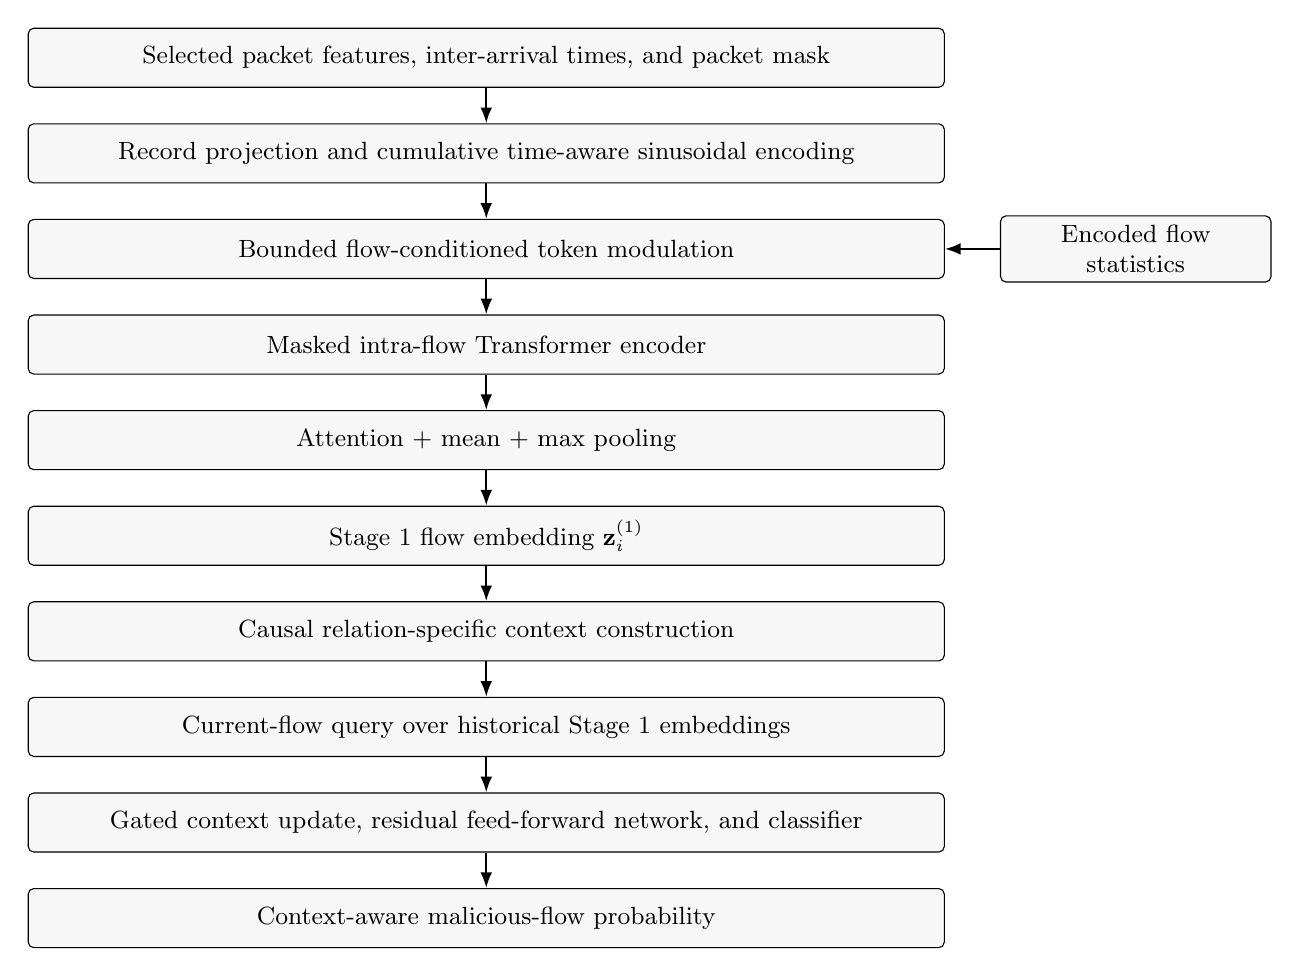
\begin{tikzpicture}[
        node distance=4.5mm,
        block/.style={draw, rectangle, rounded corners=2pt, align=center,
                      text width=11.4cm, minimum height=7.5mm, fill=black!3,
                      font=\small},
        side/.style={draw, rectangle, rounded corners=2pt, align=center,
                     text width=3.2cm, minimum height=8mm, fill=black!3,
                     font=\small},
        arrow/.style={-{Latex[length=2mm]},thick}
    ]
        \node[block] (packet) {Selected packet features, inter-arrival times, and packet mask};
        \node[block, below=of packet] (projection) {Record projection and cumulative time-aware sinusoidal encoding};
        \node[block, below=of projection] (film) {Bounded flow-conditioned token modulation};
        \node[side, right=7mm of film] (flow) {Encoded flow\\statistics};
        \node[block, below=of film] (encoder) {Masked intra-flow Transformer encoder};
        \node[block, below=of encoder] (pool) {Attention + mean + max pooling};
        \node[block, below=of pool] (z) {Stage~1 flow embedding $\mathbf{z}^{(1)}_i$};
        \node[block, below=of z] (context) {Causal relation-specific context construction};
        \node[block, below=of context] (query) {Current-flow query over historical Stage~1 embeddings};
        \node[block, below=of query] (gate) {Gated context update, residual feed-forward network, and classifier};
        \node[block, below=of gate] (output) {Context-aware malicious-flow probability};

        \draw[arrow] (packet) -- (projection);
        \draw[arrow] (projection) -- (film);
        \draw[arrow] (flow) -- (film);
        \draw[arrow] (film) -- (encoder);
        \draw[arrow] (encoder) -- (pool);
        \draw[arrow] (pool) -- (z);
        \draw[arrow] (z) -- (context);
        \draw[arrow] (context) -- (query);
        \draw[arrow] (query) -- (gate);
        \draw[arrow] (gate) -- (output);
    \end{tikzpicture}
    \caption{Detailed architecture of the proposed two-stage detector. The
    statistical branch conditions Stage~1 packet tokens, while Stage~2 uses the
    target flow as the query and historical flows as keys and values.}
    \label{fig:method_architecture}
\end{figure}

\section{Stage~1: Intra-Flow Time-Aware Representation}
\label{subsec:method_stage1}

Stage~1 transforms a variable-length packet sequence into one flow embedding.
Its principal configuration consists of a record projection, time-aware
sinusoidal encoding, flow-conditioned token modulation, a pre-normalized
Transformer encoder, hybrid mask-aware pooling, and a two-class prediction
head.

\subsection{Packet-Record Projection}
\label{subsubsec:packet_projection}

For packet position $t$, the preprocessed feature vector
$\mathbf{x}_{i,t}\in\mathbb{R}^{d_p}$ is projected to the model dimension:

\begin{equation}
    \mathbf{e}_{i,t}
    =\operatorname{LN}
    \left(W_p\mathbf{x}_{i,t}+\mathbf{b}_p\right),
    \qquad
    \mathbf{e}_{i,t}\in\mathbb{R}^{d}.
    \label{eq:record_projection}
\end{equation}

The implementation permits an MLP projection, but the principal configuration
uses one linear projection followed by layer normalization. Categorical packet
fields have already been one-hot encoded, numerical fields have been transformed
and robustly scaled, and binary fields remain in $\{0,1\}$ as described in
Section~\ref{sec:dataset_preprocessing}.

\subsection{Cumulative Time-Aware Encoding}
\label{subsubsec:time_aware_encoding}

Conventional sinusoidal positional encoding represents packet order but cannot
distinguish two adjacent packets separated by microseconds from two adjacent
packets separated by seconds. Stage~1 therefore combines ordinal position with
cumulative elapsed time. The preprocessing pipeline stores

\begin{equation}
    u_{i,t}=\log\left(1+\Delta\tau_{i,t}\right),
    \label{eq:stored_log_iat}
\end{equation}

where $\Delta\tau_{i,t}$ is the nonnegative microsecond inter-arrival time from
the previous packet in the same bidirectional flow. Inside the model, the
interval is reconstructed and masked:

\begin{equation}
    \widehat{\Delta\tau}_{i,t}
    =m_{i,t}\max\left(0,\exp(u_{i,t})-1\right).
    \label{eq:reconstructed_iat}
\end{equation}

The cumulative elapsed time and its smoothed logarithm are

\begin{align}
    c_{i,t} &= \sum_{k=1}^{t}\widehat{\Delta\tau}_{i,k},\\
    p_{i,t} &= \log\left(1+c_{i,t}+\alpha\right),
    \qquad \alpha=10^{-7}.
    \label{eq:cumulative_time_feature}
\end{align}

Let the zero-based packet position be $q_t=t-1$. The combined coordinate is
$r_{i,t}=q_t+p_{i,t}$. For channel pair $j$, the time-aware encoding is

\begin{align}
    \operatorname{TE}_{i,t,2j}
    &=\sin\left(
        \frac{r_{i,t}}{10000^{2j/d}}
      \right),\\
    \operatorname{TE}_{i,t,2j+1}
    &=\cos\left(
        \frac{r_{i,t}}{10000^{2j/d}}
      \right).
    \label{eq:time_aware_sinusoid}
\end{align}

Padding positions receive a zero encoding. The encoded packet token is

\begin{equation}
    \widetilde{\mathbf{e}}_{i,t}
    =\operatorname{Dropout}
    \left(
        \mathbf{e}_{i,t}+m_{i,t}\operatorname{TE}_{i,t}
    \right).
    \label{eq:time_encoded_packet}
\end{equation}

This construction follows the time-aware Transformer principle used in GTID
\cite{Han2023GTID}, but it is applied here to structured, payload-content-free
packet metadata. Position-only and time-only modes are retained as ablations.
In the time-only mode, $r_{i,t}=p_{i,t}$; in the position-only mode,
$r_{i,t}=q_t$.

\subsection{Flow-Statistics Encoder}
\label{subsubsec:flow_encoder}

The separately preprocessed statistical flow vector $\mathbf{s}_i$ is mapped
to the packet-model dimension through a bottleneck encoder:

\begin{equation}
    \mathbf{f}_i
    =\operatorname{LN}_2
    \left(
        W_{f,2}\,
        \operatorname{Dropout}
        \left(
            \operatorname{GELU}
            \left(
                \operatorname{LN}_1(W_{f,1}\mathbf{s}_i+\mathbf{b}_{f,1})
            \right)
        \right)
        +\mathbf{b}_{f,2}
    \right).
    \label{eq:flow_feature_encoder}
\end{equation}

The principal bottleneck dimension is 32 and the output dimension is 128. The
bottleneck limits the capacity of the aggregate-feature branch and reduces the
risk that high-dimensional flow statistics overwhelm packet-sequence evidence.

\subsection{Bounded Flow-Conditioned Token Modulation}
\label{subsubsec:token_film}

The principal Stage~1 fusion mode is inspired by feature-wise linear modulation
(FiLM), in which conditioning information produces feature-specific affine
parameters \cite{Perez2018FiLM}. From the flow representation, a small network
generates

\begin{equation}
    [\boldsymbol{\gamma}_i;\boldsymbol{\beta}_i]
    =G_f(\mathbf{f}_i),
    \qquad
    \boldsymbol{\gamma}_i,\boldsymbol{\beta}_i\in\mathbb{R}^{d}.
    \label{eq:film_parameters}
\end{equation}

For each packet token, the raw flow-conditioned residual is

\begin{equation}
    \mathbf{r}^{\mathrm{raw}}_{i,t}
    =\eta
    \left(
        \boldsymbol{\gamma}_i\odot\widetilde{\mathbf{e}}_{i,t}
        +\boldsymbol{\beta}_i
    \right),
    \qquad
    \eta=\sigma(a),quad a_{0}=-5,
    \label{eq:film_raw_residual}
\end{equation}

where $\odot$ denotes element-wise multiplication. The initial scale is
$\sigma(-5)\approx0.0067$. In addition, the residual is constrained relative
to the norm of its packet token. With the configured maximum residual ratio
$\rho=0.13$,

\begin{align}
    \lambda_{i,t}
    &=\min\left(
        1,
        \frac{\rho\|\widetilde{\mathbf{e}}_{i,t}\|_2}
             {\|\mathbf{r}^{\mathrm{raw}}_{i,t}\|_2+\epsilon}
      \right),\\
    \mathbf{e}^{F}_{i,t}
    &=\widetilde{\mathbf{e}}_{i,t}
      +\lambda_{i,t}\mathbf{r}^{\mathrm{raw}}_{i,t}.
    \label{eq:bounded_token_film}
\end{align}

The final layer producing $\boldsymbol{\gamma}_i$ and
$\boldsymbol{\beta}_i$ is initialized to zero. The model therefore begins as
the packet-only branch and learns a bounded statistical correction. This is
particularly useful when aggregate statistics are predictive but potentially
noisy or capture-specific.

The terminology is important. Because the statistical vector is encoded in a
separate branch but modulates packet tokens before self-attention, the principal
configuration is most precisely described as \emph{separate-branch conditional
intermediate fusion}. It is not strict post-pooling late fusion. A post-pooling
gated fusion implementation is available as an alternative, but the reported
principal Scheme~C configuration uses the bounded token-FiLM mechanism in
Equation~\ref{eq:bounded_token_film}.

\subsection{Masked Transformer Encoder}
\label{subsubsec:stage1_transformer}

The conditioned sequence
$\mathbf{E}^{F}_i\in\mathbb{R}^{L\times d}$ is processed by a stack of
pre-normalized Transformer encoder layers. For layer $\ell$,

\begin{align}
    \mathbf{A}^{\ell}_i
    &=\operatorname{MHA}
      \left(
        \operatorname{LN}(\mathbf{H}^{\ell-1}_i),
        \operatorname{LN}(\mathbf{H}^{\ell-1}_i),
        \operatorname{LN}(\mathbf{H}^{\ell-1}_i);
        \mathbf{m}_i
      \right),\\
    \overline{\mathbf{H}}^{\ell}_i
    &=\mathbf{H}^{\ell-1}_i
      +\operatorname{Dropout}(\mathbf{A}^{\ell}_i),\\
    \mathbf{H}^{\ell}_i
    &=\overline{\mathbf{H}}^{\ell}_i
      +\operatorname{FFN}
       \left(\operatorname{LN}(\overline{\mathbf{H}}^{\ell}_i)\right),
    \label{eq:stage1_transformer_layer}
\end{align}

where $\mathbf{H}^{0}_i=\mathbf{E}^{F}_i$. Each attention head uses scaled
dot-product attention

\begin{equation}
    \operatorname{Attn}(Q,K,V)
    =\operatorname{softmax}
      \left(
        \frac{QK^{\top}}{\sqrt{d_h}}+M_i
      \right)V,
    \label{eq:scaled_dot_product_attention}
\end{equation}

where $M_i$ assigns negative infinity to padded key positions. The feed-forward
network uses GELU activation. The principal model has two encoder layers, four
attention heads, model dimension 128, feed-forward dimension 256, and dropout
0.15.

No causal mask is used inside Stage~1: all retained packets of the completed or
truncated flow can attend to one another. Consequently, Stage~1 is a
flow-level classifier, not a claim of packet-by-packet early detection. Padding
is excluded from attention keys and from the subsequent pooling operation.

\subsection{Hybrid Mask-Aware Pooling}
\label{subsubsec:hybrid_pooling}

The packet states are reduced using three complementary summaries. First, a
learned attention score is computed for each valid token:

\begin{align}
    a_{i,t}
    &=\mathbf{w}_{a,2}^{\top}
      \operatorname{GELU}
      \left(W_{a,1}\mathbf{h}_{i,t}+\mathbf{b}_{a,1}\right)+b_{a,2},\\
    \omega_{i,t}
    &=\frac{m_{i,t}\exp(a_{i,t})}
      {\sum_{k=1}^{L}m_{i,k}\exp(a_{i,k})},\\
    \mathbf{z}^{\mathrm{att}}_i
    &=\sum_{t=1}^{L}\omega_{i,t}\mathbf{h}_{i,t}.
    \label{eq:stage1_attention_pooling}
\end{align}

The masked mean and maximum are

\begin{align}
    \mathbf{z}^{\mathrm{mean}}_i
    &=\frac{\sum_{t=1}^{L}m_{i,t}\mathbf{h}_{i,t}}
            {\max(1,\sum_{t=1}^{L}m_{i,t})},\\
    \mathbf{z}^{\mathrm{max}}_i
    &=\max_{t:m_{i,t}=1}\mathbf{h}_{i,t}.
    \label{eq:mean_max_pooling}
\end{align}

The final Stage~1 embedding combines all three:

\begin{equation}
    \mathbf{z}^{(1)}_i
    =\operatorname{Dropout}
      \left(
        \operatorname{GELU}
        \left(
          \operatorname{LN}
          \left(
            W_o
            [\mathbf{z}^{\mathrm{att}}_i;
             \mathbf{z}^{\mathrm{mean}}_i;
             \mathbf{z}^{\mathrm{max}}_i]
            +\mathbf{b}_o
          \right)
        \right)
      \right).
    \label{eq:hybrid_pooling}
\end{equation}

Attention pooling can emphasize a small number of informative packets, mean
pooling represents overall behavior, and max pooling preserves strong local
activations. Their concatenation is projected back to dimension $d$ so Stage~2
receives one consistently sized vector per flow.

The Stage~1 class logits are

\begin{equation}
    \boldsymbol{\ell}^{(1)}_i
    =h_1(\mathbf{z}^{(1)}_i),
    \qquad
    \mathbf{p}^{(1)}_i
    =\operatorname{softmax}(\boldsymbol{\ell}^{(1)}_i).
    \label{eq:stage1_classifier}
\end{equation}

The exported embedding is taken before the final two-class layer. It therefore
retains information useful for contextual refinement rather than reducing each
flow to a single probability.

\subsection{Stage~1 Fusion Variants}
\label{subsubsec:stage1_variants}

The implementation supports the three controlled variants in
Table~\ref{tab:stage1_fusion_variants}. They share the same packet features,
sequence policy, split, Transformer capacity, training procedure, and classifier
unless an experiment explicitly states otherwise.

\begin{table}[H]
    \centering
    \caption{Stage~1 packet/flow integration variants.}
    \label{tab:stage1_fusion_variants}
    \small
    \begin{tabular}{@{}p{1.1cm}p{3.1cm}p{8.9cm}@{}}
        \toprule
        Scheme & Input structure & Integration mechanism \\
        \midrule
        A & Packet + repeated flow statistics & The transformed flow vector is
        concatenated to every packet before record projection. \\
        B & Packet only & The flow-statistics branch is disabled; this isolates
        packet order and time-aware encoding. \\
        C & Packet + separate flow branch & The flow vector is encoded once and
        conditionally modulates packet tokens through bounded token-FiLM. This
        is the principal proposed Stage~1 configuration. \\
        \bottomrule
    \end{tabular}
\end{table}

\section{Stage~2: Causal Inter-Flow Context Modelling}
\label{subsec:method_stage2}

Stage~2 asks whether a target flow should be interpreted differently when
recent related behavior is available. It operates only on Stage~1 embeddings
and context metadata. Raw packet fields, flow statistics, and labels of
historical flows are not loaded into the Stage~2 input.

\subsection{Embedding Interface and Chronological Order}
\label{subsubsec:embedding_interface}

Stage~1 exports, for each split,

\begin{equation}
    \left(
      \operatorname{flow\_id}_i,
      y_i,
      \mathbf{z}^{(1)}_i,
      t_i^{0},u_i,v_i,\rho_i
    \right),
    \label{eq:stage1_export_tuple}
\end{equation}

where $t_i^{0}$ is the flow start time, $u_i$ and $v_i$ are source and
destination identifiers, and $\rho_i$ is the split. Stage~2 validates unique
flow identifiers, concatenates the split files, and stably sorts by
$(t_i^{0},\operatorname{flow\_id}_i)$. The embedding rows are reordered with
the metadata so their alignment is preserved.

Training embeddings are exported with a deterministic, non-sampled loader.
This is essential because the weighted training sampler draws with replacement;
using it for export would duplicate some flows and omit others. The weighted
sampler is used only for optimization batches.

\subsection{Relation-Specific Causal Contexts}
\label{subsubsec:context_relations}

The context builder scans the sorted flows once from past to future. Before
adding target flow $i$ to any history, it retrieves eligible earlier indices.
The four evaluated relations are defined in
Table~\ref{tab:context_relations}.

\begin{table}[H]
    \centering
    \caption{Stage~2 context relations.}
    \label{tab:context_relations}
    \small
    \begin{tabular}{@{}p{3.0cm}p{4.0cm}p{7.1cm}@{}}
        \toprule
        Method & Eligibility condition for $j<i$ & Interpretation \\
        \midrule
        \methodfield{time_only} & Always eligible & Most recent flows globally,
        regardless of endpoint identity. \\
        \methodfield{source_host} & $u_j=u_i$ & Earlier flows initiated by the
        same source identifier. \\
        \methodfield{destination_host} & $v_j=v_i$ & Earlier flows directed to
        the same destination identifier. \\
        \methodfield{endpoint} &
        $\{u_j,v_j\}\cap\{u_i,v_i\}\neq\varnothing$ & Earlier flows sharing at
        least one endpoint in either role. \\
        \bottomrule
    \end{tabular}
\end{table}

For relation $r$, let

\begin{equation}
    \mathcal{A}^{(r)}_i
    =\left\{j<i:R_r(i,j)=1\right\}.
    \label{eq:method_eligible_context}
\end{equation}

After split-policy filtering and deduplication, the most recent $W-1$ indices
are retained:

\begin{equation}
    \mathcal{C}^{(r)}_i
    =\operatorname{Recent}_{W-1}
      \left(\mathcal{A}^{(r)}_i\right).
    \label{eq:recent_context}
\end{equation}

The current flow is then appended, producing
Equation~\ref{eq:method_stage2_input}. Histories are updated only after this
sequence has been built, which prevents self-inclusion and future leakage. The
principal context policy is \methodfield{online}: validation flows may use
earlier training flows, and test flows may use earlier training, validation,
and test flows, but never a future flow. This simulates persistent detector
state across chronological deployment. No historical label is exposed.

The term \methodfield{time_only} means chronological global recency. It does
not mean that continuous inter-flow time gaps are supplied to Stage~2. In the
current implementation, Stage~2 encodes relative context age, while explicit
microsecond timing is modelled inside Stage~1.

The collate function left-pads short sequences so the target remains at the last
valid position:

\begin{equation}
    [\mathrm{PAD},\ldots,\mathrm{PAD},
      \mathbf{z}^{(1)}_{j_1},\ldots,
      \mathbf{z}^{(1)}_{j_{K_i}},
      \mathbf{z}^{(1)}_i].
    \label{eq:left_padded_context}
\end{equation}

The accompanying Boolean mask makes the physical padding positions irrelevant
to positional encoding and attention.

\subsection{Context-Age Positional Encoding}
\label{subsubsec:context_age_encoding}

If a target has $K_i$ historical tokens, the target receives age 0, the most
recent historical flow receives age 1, and the oldest retained flow receives
age $K_i$. Let $a_{i,k}$ denote this age index. Stage~2 adds a conventional
sinusoidal encoding

\begin{align}
    \operatorname{PE}_{i,k,2j}
    &=\sin\left(
        \frac{a_{i,k}}{10000^{2j/d}}
      \right),\\
    \operatorname{PE}_{i,k,2j+1}
    &=\cos\left(
        \frac{a_{i,k}}{10000^{2j/d}}
      \right).
    \label{eq:stage2_age_encoding}
\end{align}

Unlike absolute tensor positions, age values are invariant to the amount of
left padding. This allows the same target and history order to receive the same
encoding in batches with different sequence lengths.

\subsection{Target-Query Gated Multi-Head Attention}
\label{subsubsec:target_query_attention}

The principal Stage~2 model is
\methodfield{target_query_gated}. Rather than allowing every historical token
to attend to every other historical token, it uses the current flow as one
query over the eligible history. Let $\mathbf{c}_i$ be the projected current
Stage~1 embedding and let
$\widetilde{\mathbf{H}}_i\in\mathbb{R}^{K_i\times d}$ contain age-encoded
historical embeddings. For attention head $h$,

\begin{align}
    \mathbf{q}^{h}_i
    &=W_Q^{h}\operatorname{LN}
      \left(\mathbf{c}_i+\operatorname{PE}(0)\right),\\
    \mathbf{K}^{h}_i
    &=\operatorname{LN}(\widetilde{\mathbf{H}}_i)W_K^{h},\\
    \mathbf{V}^{h}_i
    &=\operatorname{LN}(\widetilde{\mathbf{H}}_i)W_V^{h},\\
    \mathbf{h}^{h}_i
    &=\operatorname{softmax}
      \left(
        \frac{\mathbf{q}^{h}_i(\mathbf{K}^{h}_i)^{\top}}
             {\sqrt{d_h}}+M_i
      \right)
      \mathbf{V}^{h}_i.
    \label{eq:target_query_attention}
\end{align}

The head outputs are concatenated and projected to obtain the historical
summary $\mathbf{h}_i$. If no eligible historical flow exists,
$\mathbf{h}_i=\mathbf{0}$. This explicit fallback prevents a fabricated
padding token from contributing context.

The model compares the current representation and context summary through
difference and multiplicative interactions:

\begin{align}
    \mathbf{r}_i
    &=[\mathbf{c}_i;\mathbf{h}_i;
       \mathbf{c}_i-\mathbf{h}_i;
       \mathbf{c}_i\odot\mathbf{h}_i],\\
    \mathbf{v}_i
    &=[\mathbf{h}_i;
       \mathbf{c}_i-\mathbf{h}_i;
       \mathbf{c}_i\odot\mathbf{h}_i].
    \label{eq:target_context_interactions}
\end{align}

A dimension-wise gate and context update are then computed:

\begin{align}
    \mathbf{g}_i&=\sigma(G(\mathbf{r}_i)),\\
    \mathbf{d}_i&=U(\mathbf{v}_i),\\
    \mathbf{f}_i&=\operatorname{LN}
      \left(\mathbf{c}_i+\mathbf{g}_i\odot\mathbf{d}_i\right).
    \label{eq:gated_context_update}
\end{align}

When no history exists, both $\mathbf{g}_i$ and $\mathbf{d}_i$ are set to zero,
so the model reduces to the current-flow representation. Finally, a residual
feed-forward block produces

\begin{align}
    \mathbf{z}^{(2)}_i
    &=\operatorname{LN}
      \left(
        \mathbf{f}_i+\operatorname{FFN}(\mathbf{f}_i)
      \right),\\
    \boldsymbol{\ell}^{(2)}_i
    &=h_2(\mathbf{z}^{(2)}_i).
    \label{eq:stage2_output}
\end{align}

The target-query formulation preserves a strong current-flow path and lets
context act as a learned correction. Its attention-score matrix grows linearly
with $W$ because it contains one query, whereas full self-attention constructs
an $W\times W$ score matrix. This makes a window of 128 flows practical while
retaining multi-head retrieval from historical behavior.

\subsection{Stage~2 Control Models}
\label{subsubsec:stage2_controls}

To distinguish gains from context selection from gains caused merely by an
additional classifier, all control models consume the same Stage~1 embeddings,
context indices, left-padding convention, train/validation/test partitions,
and optimization pipeline.

\begin{itemize}[leftmargin=*]
    \item \textbf{No-context MLP} selects only the final valid target token and
    applies the same projection/classification style. It is the direct control
    for whether historical flows add useful information.

    \item \textbf{Vanilla Stage~2 Transformer} applies self-attention to the
    complete context sequence and classifies the last valid token. It tests
    whether all-to-all context interaction is preferable to target-query
    retrieval.

    \item \textbf{LSTM and GRU} use packed, right-compacted versions of the same
    context sequences and classify the last recurrent state
    \cite{Hochreiter1997LSTM,Cho2014GRU}.

    \item \textbf{CNN+LSTM} applies parallel one-dimensional convolutions with
    kernel sizes 3, 5, and 7, projects their concatenated outputs, and then uses
    an LSTM. This control combines local pattern extraction with recurrent
    sequence modelling \cite{Kim2014CNN,Hochreiter1997LSTM}.
\end{itemize}

These models are comparison baselines rather than components simultaneously
active in the proposed target-query model.

\section{Imbalance-Aware Sequential Training}
\label{subsec:method_training}

\subsection{Focal Objective and Controlled Sampling}
\label{subsubsec:focal_training}

Both stages use two-class softmax outputs and focal loss. For a sample with
label $y_i$ and predicted probability $p_{i,y_i}$,

\begin{equation}
    \mathcal{L}_{\mathrm{focal}}
    =-\frac{1}{B}
      \sum_{i=1}^{B}
      \alpha_{y_i}
      \left(1-p_{i,y_i}\right)^{\gamma}
      \log p_{i,y_i}.
    \label{eq:method_focal_loss}
\end{equation}

Focal loss reduces the influence of easily classified examples and was
originally proposed for severe foreground/background imbalance
\cite{Lin2017FocalLoss}. The principal configuration uses $\gamma=1$ and no
label smoothing. Stage~1 applies mild class weights $[1,1.25]$; Stage~2 uses
near-uniform weights $[1,1.01]$.

Training batches are additionally formed by a controlled weighted sampler. If
$n_0$ and $n_1$ are the training counts and the desired expected positive
fraction is $q$, each negative and positive example receives

\begin{equation}
    w_0=\frac{1-q}{n_0},
    \qquad
    w_1=\frac{q}{n_1}.
    \label{eq:controlled_sampler}
\end{equation}

Sampling is performed with replacement for exactly the original number of
training examples per epoch. The principal values are $q=0.09$ for Stage~1 and
$q=0.05$ for Stage~2. These values increase minority exposure relative to the
natural 3.945\% prevalence without forcing an artificial 50/50 training
distribution. Validation and test loaders never use weighted sampling.

\subsection{Optimization and Model Selection}
\label{subsubsec:optimization}

Both stages are optimized with AdamW, which decouples weight decay from the
adaptive gradient update \cite{Loshchilov2019AdamW}. Stage~1 uses learning rate
$10^{-4}$, weight decay $10^{-4}$, batch size 128, gradient-norm clipping at
1.0, and mixed-precision training when CUDA is available. A
ReduceLROnPlateau scheduler monitors validation PR-AUC, halves the learning rate
after five unimproved epochs, and does not reduce it below $10^{-6}$. Training
stops after 25 epochs without improvement, up to a maximum of 500 epochs.

Stage~2 uses learning rate $3\times10^{-5}$, weight decay
$3\times10^{-4}$, batch size 128, gradient-norm clipping at 0.5, and mixed
precision on CUDA. The first five epochs linearly warm the learning rate from
5\% to 100\% of its configured value. Cosine annealing then reduces it to 1\%
of the initial rate. Early stopping patience is 15 epochs with a maximum of 500
epochs.

The best checkpoint in each stage is selected by validation PR-AUC. This
threshold-independent criterion is appropriate for the imbalanced data and
avoids selecting a checkpoint from accuracy dominated by label~0
\cite{SaitoRehmsmeier2015}. The test partition is not used to choose the model.
% 
% \subsection{Sequential Stage Training and Embedding Export}
% \label{subsubsec:sequential_training}

% The complete training procedure is:

% \begin{enumerate}[label=\textbf{Step \arabic*:},leftmargin=*]
%     \item Fit the Stage~1 preprocessor only on the training partition and
%     transform all partitions with the frozen preprocessing state.

%     \item Train Stage~1 using the weighted training loader. Select the best
%     checkpoint by validation PR-AUC and restore that checkpoint.

%     \item Export exactly one Stage~1 embedding per flow using deterministic,
%     non-sampled loaders. Store the flow identifier, label, split, start time,
%     source identifier, and destination identifier with the embedding.

%     \item Concatenate and chronologically sort the Stage~1 outputs. Construct
%     causal context indices using only metadata and prior indices.

%     \item Train Stage~2 while treating Stage~1 embeddings as fixed inputs.
%     Select and restore the best Stage~2 checkpoint using validation PR-AUC.

%     \item Select a decision threshold on validation predictions and apply that
%     fixed threshold once to the test predictions.
% \end{enumerate}

% The current implementation does not back-propagate Stage~2 gradients into
% Stage~1. Sequential training makes the source of an improvement auditable: a
% Stage~2 gain is attributable to contextual modelling over a fixed representation,
% not to an unreported change in the packet encoder.

% \subsection{Validation-Selected Decision Threshold}
% \label{subsubsec:decision_threshold}

% For class-1 probability $p_i$, the prediction is

% \begin{equation}
%     \widehat{y}_i=\mathbb{I}[p_i\geq\delta^{*}].
%     \label{eq:method_decision_rule}
% \end{equation}

% The principal implementation selects $\delta^{*}$ by maximizing class-1 F1 on
% the validation partition. Stage~2 searches 199 thresholds between 0.01 and
% 0.99. The selected threshold is then frozen for test evaluation. Macro-F1 is
% the primary reported aggregate F1 metric, while class-1 precision, recall, and
% F1 are reported separately to make the threshold trade-off explicit. A
% test-optimized threshold may be computed only as a clearly labelled diagnostic
% oracle and must not be reported as deployable test performance. This separation
% follows standard guidance against test-set adaptation in security machine
% learning \cite{Arp2022DosDonts}.

\section{Principal Configuration}
\label{subsec:principal_configuration}

Table~\ref{tab:principal_method_config} records the architecture used for the
principal experiments. Values changed by an ablation, such as packet sequence
length, truncation strategy, context relation, 有问题
% or Stage~2 encoder type, must be
% reported with that experiment rather than silently replacing this table.

\begin{table}[H]
    \centering
    \caption{Principal architecture and optimization configuration.}
    \label{tab:principal_method_config}
    \small
    \begin{tabular}{@{}p{2.0cm}p{4.4cm}p{7.6cm}@{}}
        \toprule
        Stage & Component & Principal value \\
        \midrule
        Stage~1 & Packet sequence & $L=128$, head selection, right padding \\
        Stage~1 & Packet encoder & $d=128$, 4 heads, 2 Transformer layers,
        FFN dimension 256, dropout 0.15 \\
        Stage~1 & Time encoding & Position + cumulative log-time,
        $\alpha=10^{-7}$ \\
        Stage~1 & Statistical branch & Bottleneck dimension 32, token-FiLM,
        initial scale logit $-5$, residual cap $\rho=0.13$ \\
        Stage~1 & Pooling & Learned attention + masked mean + masked max \\
        Stage~1 & Optimization & AdamW, $10^{-4}$ learning rate,
        $10^{-4}$ weight decay, batch 128, focal $\gamma=1$,
        sampled positive fraction 0.09 \\
        \midrule
        Stage~2 & Main encoder & Target-query gated multi-head attention \\
        Stage~2 & Context & Source-host in the principal/best configuration;
        time-only, destination-host, and endpoint are controlled comparisons \\
        Stage~2 & Context policy & $W=128$ including target, online causal
        history, deduplication, left padding \\
        Stage~2 & Representation & $d=128$, 4 heads, age positional encoding,
        FFN dimension 256, dropout 0.25 \\
        Stage~2 & Optimization & AdamW, $3\times10^{-5}$ learning rate,
        $3\times10^{-4}$ weight decay, batch 128, focal $\gamma=1$,
        sampled positive fraction 0.05 \\
        Both & Reproducibility & Random seed 130; validation PR-AUC checkpoint
        selection; validation-only threshold selection \\
        \bottomrule
    \end{tabular}
\end{table}

% \section{Computational Properties}
% \label{subsec:method_complexity}

% For one Stage~1 flow, the self-attention score computation in each layer has
% time and memory complexity $O(L^2d)$ and $O(L^2)$, respectively, while the
% feed-forward block costs $O(Ld d_{\mathrm{ff}})$. The statistical encoder and
% token-FiLM modulation are linear in $L$. Fixing $L=128$ therefore bounds both
% memory and inference cost independently of the original packet count.

% For Stage~2, context construction is performed once by maintaining bounded
% global and host-indexed histories. The target-query attention map contains
% $W-1$ scores per head rather than $W^2$ scores, giving attention-map time and
% memory $O(Wd)$ and $O(W)$ per target, excluding the linear projections. The
% bounded context window prevents high-activity hosts from producing unbounded
% sequences.

% The hierarchy also permits deployment choices that a monolithic model would
% not. Stage~1 embeddings can be cached once per flow, and alternative Stage~2
% relations or encoders can be evaluated without reprocessing packets. The cost
% is that Stage~2 performance depends on the fixed Stage~1 representation and
% that the current sequential implementation is not jointly optimized end to end.

\section{Methodological Summary}
\label{subsec:method_summary}

The proposed method first learns a packet-order- and time-aware flow
representation, conservatively conditions it on aggregate flow statistics, and
then refines the decision using causal histories of related flow embeddings.
The main Stage~1 contribution is the combination of cumulative time-aware
encoding, bounded flow-conditioned token modulation, and hybrid pooling. The
main Stage~2 contribution is a relation-controlled target-query attention
mechanism with a gated residual update and an exact no-history fallback. The
strict separation among predictors, context metadata, and labels, together
with chronological context construction and validation-only model selection,
keeps the method aligned with realistic temporal evaluation.


% Experimental Methodology chapter for:
% A Hierarchical Time-Aware Transformer for Flow-Level Network Intrusion Detection
%
% Required packages already used by the thesis:
%   amsmath, booktabs, multirow, array, graphicx
% Recommended in the main preamble:
%   \usepackage{amssymb}
%
% Replace the five environment macros below with values copied from the
% environment in which the final reported runs were executed. Leaving these
% values unresolved in a submitted thesis would make the efficiency results
% difficult to reproduce.
\providecommand{\ExpGPU}{\textit{[insert accelerator model and memory]}}
\providecommand{\ExpCPU}{\textit{[insert CPU model and RAM]}}
\providecommand{\ExpOS}{\textit{[insert operating system or Colab runtime]}}
\providecommand{\ExpSoftware}{\textit{[insert Python, PyTorch, CUDA, and scikit-learn versions]}}
\providecommand{\ExpSuricata}{\textit{[insert Suricata version and custom-plugin revision]}}

% Experimental Methodology chapter for:
% A Hierarchical Time-Aware Transformer for Flow-Level Network Intrusion Detection
%
% Required packages already used by the thesis:
%   amsmath, booktabs, multirow, array, graphicx
% Recommended in the main preamble:
%   \usepackage{amssymb}
%
% The platform and purchased allocation are known. Replace the remaining
% environment macros with values captured from each final Colab runtime.
% In particular, do not replace \ExpGPU with only "GPU": record T4 or L4.
\providecommand{\ExpPlatform}{Google Colaboratory Pro+}
\providecommand{\ExpComputeBudget}{600 purchased compute units}
\providecommand{\ExpGPU}{NVIDIA T4 (16~GB) or NVIDIA L4 (24~GB); exact model recorded per run}
\providecommand{\ExpCPU}{\textit{[insert CPU model and RAM]}}
\providecommand{\ExpOS}{Google Colab hosted Linux runtime; \textit{[insert runtime image details]}}
\providecommand{\ExpSoftware}{\textit{[insert Python, PyTorch, CUDA, and scikit-learn versions]}}
\providecommand{\ExpSuricata}{\textit{[insert Suricata version and custom-plugin revision]}}

\chapter{Experimental Methodology}
\label{sec:experimental_methodology}

This chapter defines the protocol used to evaluate the proposed hierarchical
detector. Its purpose is to separate model development from final evaluation,
to make comparisons between alternatives fair, and to ensure that every
reported number can be traced to a dataset manifest, model configuration,
checkpoint, decision threshold, and random seed. This separation is especially
important in intrusion detection because temporal leakage, class imbalance,
and repeated use of the test set can produce highly optimistic conclusions
\cite{SommerPaxson2010,Arp2022DosDonts}.

To avoid duplicating earlier chapters, this chapter does not redefine the raw
packet and flow schemas, the mathematical detection problem, or the internal
layers of the proposed models. Dataset provenance and transformations are
given in Section~\ref{sec:dataset_preprocessing}, the research questions and
notation in Section~\ref{sec:problem_formulation}, and the architecture in
Section~\ref{sec:proposed_methodology}. The present chapter specifies only the
experimental comparisons, controls, optimization protocol, metrics,
statistical analysis, and computational measurement needed to test that
methodology.

The evaluation is organized around the two research questions mapped to
controlled comparisons in Table~\ref{tab:rq_mapping}. Stage~1 experiments
address whether ordered packet records,
continuous-time information, and flow statistics improve the representation
of an individual flow. Stage~2 experiments address whether causal context from
earlier related flows improves the classification of the current flow. In both
stages, macro-F1 is the primary threshold-dependent metric. Macro-precision,
macro-recall, class-1 performance, ROC-AUC, PR-AUC, the confusion matrix, and
the false-positive rate (FPR) provide complementary evidence. Parameter count,
training time, and inference time are reported to distinguish predictive gains
from increases in computational cost.

\section{Dataset Partition and Leakage Controls}
\label{subsec:experimental_data_protocol}

All experiments use the aligned flow manifest constructed in
Section~\ref{sec:dataset_preprocessing}. The PCAP provenance, exact packet and
flow counts, label distribution, selected predictors, and exclusions are
reported once in Sections~\ref{subsec:raw_composition}--
\ref{subsec:feature_selection} and are not restated here. The experimental
invariant is that every comparison uses the same flow universe and the same
training-fitted preprocessing state unless a table explicitly identifies a
separate exploratory manifest.

\subsubsection{Chronological Hold-Out Protocol}
\label{subsubsec:chronological_holdout}

The fixed 70/10/20 chronological split and its exact counts are defined in
Table~\ref{tab:chronological_split}. Unique flows are stably ordered by
\texttt{flow\_start\_timestamp\_us}, with \texttt{flow\_id} as the
deterministic tie-breaker, and all packets from one flow remain in the same
partition. This chronological design evaluates the more deployment-like
setting in which a detector is trained on earlier traffic and applied to later
traffic, rather than allowing temporally adjacent records to be distributed
randomly across partitions \cite{SommerPaxson2010,Arp2022DosDonts}.

All data-dependent transformations are fitted using the training partition
only. These include categorical vocabularies, quantile clipping bounds,
logarithmic transformations, and robust-scaling parameters. The fitted
preprocessor is then applied without refitting to validation and test data.
Class weights and sampling probabilities are also calculated from training
labels only.

\subsubsection{Stage~2 Causality and Split Policy}
\label{subsubsec:stage2_evaluation_causality}

Stage~2 consumes embeddings exported by one frozen Stage~1 checkpoint. Its
context builder scans flows in chronological order and updates a history only
after the current example has been constructed. Consequently, the context of
flow $i$ may contain only flows with earlier timestamps; neither future
embeddings nor historical labels are retrieved. Under the principal
\texttt{online} policy, a validation example may use earlier training flows,
and a test example may use earlier training, validation, and test flows. This
simulates a continuously operating detector whose past observations remain
available, while preserving the rule that no future observation can influence
the present prediction.

All Stage~2 model comparisons use exactly the same Stage~1 embedding files,
metadata ordering, context indices, and left-padding masks. The Stage~1 encoder
is not fine-tuned during Stage~2 training. A change in Stage~1 checkpoint would
therefore constitute a new experiment rather than a Stage~2 architecture
ablation.

\section{Experimental Matrix}
\label{subsec:experimental_matrix}

The complete evaluation matrix is summarized in
Table~\ref{tab:experiment_matrix}. The matrix separates comparisons intended
to evaluate the packet encoder from comparisons intended to evaluate the full
hierarchical system.

\begin{table}[H]
    \centering
    \caption{Experimental matrix. Only the factor listed in the final column is
    changed within each experiment group.}
    \label{tab:experiment_matrix}
    \resizebox{\textwidth}{!}{%
    \begin{tabular}{@{}lllll@{}}
        \toprule
        Group & Stage & Fixed reference & Compared alternatives & Varied factor \\
        \midrule
        S1-E1 & 1 & Full chronological split & Flow MLP; packet
        sequence models; proposed Stage~1 & Encoder family \\
        S1-E2 & 1 & Scheme B, $L=128$, head & Both, position-only,
        time-only, no encoding & Temporal/order encoding \\
        S1-E3 & 1 & Both encodings, $L=128$, head & Schemes A, B, C &
        Flow-statistics integration \\
        S1-E4 & 1 & Scheme B, head & $L=8,16,32,64,128,256$ & Packet budget \\
        S1-E5 & 1 & Scheme B, $L=128$ & Head, head-tail, random &
        Truncation policy \\
        S2-E1 & 2 & Same frozen Stage~1 embeddings & No-context MLP;
        Transformer; LSTM; GRU; CNN+LSTM; proposed & Context encoder \\
        S2-E2 & 2 & Proposed model, $W=128$ & Time-only, source-host,
        destination-host, endpoint & Context relation \\
        S2-E3 & 2 & Proposed model, source-host & $W=16,32,64,128,256$ &
        Context capacity \\
        \bottomrule
    \end{tabular}%
    }
\end{table}

\subsubsection{Stage~1 Baselines}
\label{subsubsec:stage1_baselines}

The Stage~1 comparison includes the following baselines:

\begin{itemize}[leftmargin=*]
    \item \textbf{Flow-level MLP.} A multilayer perceptron consumes only the
    aggregated statistical flow vector. It provides the direct reference for
    testing whether packet-level sequence information adds value beyond
    conventional flow aggregation.

    \item \textbf{CNN1D.} Parallel one-dimensional convolutions with kernel
    sizes 3, 5, and 7 capture local packet motifs, followed by global pooling
    and classification. A second variant concatenates the log inter-arrival
    feature to each packet record. The design follows the general use of
    multi-kernel convolution for sequence classification \cite{Kim2014CNN}.

    \item \textbf{LSTM and BiLSTM.} Two-layer recurrent encoders with hidden
    width 128 and mean pooling provide unidirectional and bidirectional
    sequence references. The LSTM-with-time variant concatenates the stored
    log inter-arrival value to each packet vector
    \cite{Hochreiter1997LSTM}.

    \item \textbf{GRU.} A two-layer, width-128 GRU with mean pooling tests
    whether a lighter gated recurrent encoder is sufficient
    \cite{Cho2014GRU}.

    \item \textbf{Standard Transformer.} This control has the same packet
    projection and self-attention family as the proposed Stage~1 model but
    uses conventional order encoding without the proposed cumulative-time
    mechanism \cite{Vaswani2017}.
\end{itemize}

The recurrent and convolutional baselines use the same packet feature tensors,
sequence masks, chronological split, focal objective, sampler, optimizer
budget, validation-based checkpoint rule, and threshold-selection rule as the
proposed model \emph{within the Stage~1 model-family benchmark}. In the current
comparison trainer, every member of this benchmark, including the proposed
encoding variants, is checkpointed by validation class-1 F1 and obtains its
threshold from the validation precision-recall points. This shared rule makes
the rows within that benchmark comparable. It differs from the standalone
principal Stage~1 trainer described below, which checkpoints by validation
PR-AUC. The two protocols are therefore kept in separate tables unless all
models are rerun through one common trainer. Model capacity is not forced to be
identical because doing so can make one architecture artificially weak;
instead, trainable parameter count and runtime are reported next to predictive
performance.

\subsubsection{Stage~1 Ablations and Sensitivity Tests}
\label{subsubsec:stage1_ablation_protocol}

Four encoding variants isolate the contribution of order and elapsed time:
(i) both positional and time-aware encoding, (ii) positional encoding only,
(iii) time-aware encoding only, and (iv) neither encoding. These variants keep
the packet features and Transformer capacity unchanged. Their comparison is
particularly important because concatenating an interval value to a packet
vector is not equivalent to using elapsed time as the coordinate of a
sinusoidal sequence encoding.

Flow-statistics integration is evaluated through the three schemes defined in
Table~\ref{tab:stage1_fusion_variants}. Scheme A repeats flow statistics at
every packet position, Scheme B excludes flow statistics, and Scheme C uses a
separate flow branch with bounded token-FiLM conditioning. Scheme B is used
for packet-encoder and truncation studies because it isolates sequence
modelling from flow-statistics fusion. Scheme C is the principal complete
Stage~1 model and supplies the embeddings used by Stage~2.

Sequence-length sensitivity is measured with
$L\in\{8,16,32,64,128,256\}$ under \texttt{head} selection. Selection-policy
sensitivity fixes $L=128$ and compares \texttt{head},
\texttt{head\_tail}, and deterministic \texttt{random} subsampling. All other
settings remain unchanged. In particular, a new threshold is selected on the
validation predictions of each trained variant; the test set is not searched
for a favorable operating point.

\subsubsection{Stage~2 Baselines and Context Ablations}
\label{subsubsec:stage2_baseline_protocol}

The proposed target-query gated attention model is compared with five controls:

\begin{itemize}[leftmargin=*]
    \item \textbf{No-context MLP} classifies only the current Stage~1
    embedding and therefore measures the gain attributable to historical
    context.

    \item \textbf{Vanilla Transformer} applies full self-attention to the same
    context sequence and classifies its last valid token
    \cite{Vaswani2017}.

    \item \textbf{LSTM} and \textbf{GRU} replace attention with recurrent
    context encoders while preserving the Stage~1 inputs, context window,
    masks, and classifier protocol \cite{Hochreiter1997LSTM,Cho2014GRU}.

    \item \textbf{CNN+LSTM} applies parallel temporal convolutions with kernel
    sizes 3, 5, and 7 before a two-layer LSTM, combining local pattern
    extraction with recurrent context modelling
    \cite{Kim2014CNN,Hochreiter1997LSTM}.
\end{itemize}

For the architecture comparison, contextual baselines receive the same
\texttt{source\_host} histories with $W=128$ and the current flow included as
the last valid element. With the target included, the maximum historical
capacity is $W-1=127$ flows. The no-context model receives the same target
embedding but discards all preceding elements.

Context-relation sensitivity fixes the proposed encoder and $W=128$, then
changes only the eligibility relation among \texttt{time\_only},
\texttt{source\_host}, \texttt{destination\_host}, and \texttt{endpoint}.
Window-size sensitivity fixes \texttt{source\_host} and evaluates
$W\in\{16,32,64,128,256\}$. For each context configuration, the dataset report
records the minimum, median, mean, 95th percentile, and maximum number of valid
elements. This reveals whether a nominally larger window actually supplies
more history or is mostly padding for low-activity hosts.

\section{Training, Model Selection, and Thresholding}
\label{subsec:experimental_training_protocol}

\subsubsection{Principal Training Configuration}
\label{subsubsec:principal_training_config}

The architecture and optimization settings follow
Table~\ref{tab:principal_method_config}. The main values relevant to
experimental replication are summarized in
Table~\ref{tab:experimental_training_config}. AdamW is used in both stages to
decouple weight decay from the adaptive gradient update
\cite{Loshchilov2019AdamW}. Focal loss reduces the influence of easy examples
from the majority class \cite{Lin2017FocalLoss}.

\begin{table}[H]
    \centering
    \caption{Principal optimization configuration. Values changed in a named
    ablation are the only exceptions.}
    \label{tab:experimental_training_config}
    \begin{tabular}{@{}p{3.0cm}p{4.6cm}p{5.7cm}@{}}
        \toprule
        Setting & Stage~1 & Stage~2 \\
        \midrule
        Architecture and input & Table~\ref{tab:principal_method_config} &
        Table~\ref{tab:principal_method_config} \\
        Batch size & 128 & 128 \\
        Optimizer & AdamW & AdamW \\
        Learning rate & $1\times10^{-4}$ & $3\times10^{-5}$ \\
        Weight decay & $1\times10^{-4}$ & $3\times10^{-4}$ \\
        Gradient clipping & Global norm 1.0 & Global norm 0.5 \\
        Loss & Focal, $\gamma=1$ & Focal, $\gamma=1$ \\
        Sampler target & 9\% class-1 examples & 5\% class-1 examples \\
        Maximum epochs & 500 & 500 \\
        Early-stopping patience & 25 epochs & 15 epochs \\
        Checkpoint criterion & Validation PR-AUC & Validation PR-AUC \\
        Random seed & 130 & 130 \\
        \bottomrule
    \end{tabular}
\end{table}

The weighted sampler is used only to construct training mini-batches and draws
with replacement. Validation, test, and embedding-export loaders are
non-sampled and preserve one row per flow. This distinction prevents the
sampler from duplicating flow embeddings or altering the empirical label
distribution used for evaluation. Automatic mixed precision is enabled on
CUDA. Stage~1 reduces the learning rate when validation PR-AUC plateaus;
Stage~2 uses five warm-up epochs followed by cosine annealing.

\section{Evaluation Metrics}
\label{subsec:experimental_metrics}

The implementation uses the metric definitions provided by scikit-learn
\cite{Pedregosa2011ScikitLearn}. Label 1 is the alert-derived positive class and
label 0 is the negative class. The confusion matrix is always reported in the
following orientation:
\begin{equation}
    \mathbf{C}=
    \begin{bmatrix}
        \mathrm{TN} & \mathrm{FP}\\
        \mathrm{FN} & \mathrm{TP}
    \end{bmatrix},
    \label{eq:experimental_confusion_matrix}
\end{equation}
where rows denote true labels and columns denote predicted labels. Stating the
orientation prevents an ambiguity that is common when confusion matrices are
copied between software packages.

\subsubsection{Class-Wise and Macro-Averaged Measures}
\label{subsubsec:macro_metrics}

For class $c\in\{0,1\}$, precision, recall, and F1 are
\begin{align}
    P_c &= \frac{\mathrm{TP}_c}
    {\mathrm{TP}_c+\mathrm{FP}_c}, \\
    R_c &= \frac{\mathrm{TP}_c}
    {\mathrm{TP}_c+\mathrm{FN}_c}, \\
    F_{1,c} &= \frac{2P_cR_c}{P_c+R_c}.
    \label{eq:classwise_metrics}
\end{align}
Undefined ratios are assigned zero, matching the implementation's
\texttt{zero\_division=0} setting. The macro-averaged metrics are
\begin{align}
    P_{\mathrm{macro}} &= \frac{P_0+P_1}{2}, \\
    R_{\mathrm{macro}} &= \frac{R_0+R_1}{2}, \\
    F_{1,\mathrm{macro}} &= \frac{F_{1,0}+F_{1,1}}{2}.
    \label{eq:experimental_macro_metrics}
\end{align}

Macro-F1 is the primary F1 reported in this thesis and is denoted simply as
``F1'' in high-level result tables. It weights benign and positive classes
equally despite their different frequencies. Macro-precision and macro-recall
are the corresponding primary precision and recall measures. Because macro
averaging can conceal which error type changed, $P_1$, $R_1$, and $F_{1,1}$
are always reported alongside the macro values.

Accuracy and weighted averages are included for completeness but are treated
as secondary. On the raw dataset, an always-negative classifier would achieve
approximately $96.055\%$ accuracy while obtaining zero positive recall. High
accuracy or weighted F1 is therefore not sufficient evidence of an effective
intrusion detector.

\subsubsection{False-Positive Rate and Operational Error Counts}
\label{subsubsec:fpr_metric}

The false-positive rate is
\begin{equation}
    \mathrm{FPR}=\frac{\mathrm{FP}}{\mathrm{FP}+\mathrm{TN}},
    \label{eq:false_positive_rate}
\end{equation}
and the false-negative rate is
\begin{equation}
    \mathrm{FNR}=\frac{\mathrm{FN}}{\mathrm{FN}+\mathrm{TP}}
    =1-R_1.
    \label{eq:false_negative_rate}
\end{equation}
FPR is emphasized because even a small rate can create a large alert volume in
a high-throughput network. Each result table therefore reports both FPR and the
absolute numbers of FP and FN. For a test partition containing $N_0$ benign
flows, the expected number of false alerts at the evaluated operating point is
$N_0\times\mathrm{FPR}$.

\subsubsection{Threshold-Independent Ranking Measures}
\label{subsubsec:ranking_metrics}

ROC-AUC summarizes the true-positive rate as the false-positive rate varies
over all score thresholds \cite{Fawcett2006ROC}. It measures ranking quality
but can remain high when the negative class dominates. PR-AUC focuses on the
positive class and is therefore given greater weight for this imbalanced
dataset \cite{SaitoRehmsmeier2015}.

The code field named \texttt{pr\_auc} is computed with scikit-learn's
\texttt{average\_precision\_score}. It is therefore average precision (AP),
not trapezoidal integration of linearly interpolated precision-recall points:
\begin{equation}
    \mathrm{AP}=\sum_{k}(R_k-R_{k-1})P_k,
    \label{eq:average_precision}
\end{equation}
where $P_k$ and $R_k$ are the precision and recall at successive score
thresholds. To remain consistent with the stored result files, this thesis
uses the label ``PR-AUC (AP)'' on first mention and ``PR-AUC'' thereafter. A
random ranking has expected AP close to the class-1 prevalence, so the observed
value should be interpreted relative to the test partition's positive rate.

% \section{Statistical Reliability}
% \label{subsec:statistical_reliability}

% Neural results can vary with initialization and mini-batch order; a single
% best run can therefore overstate an architecture's advantage
% \cite{ReimersGurevych2017,Bouthillier2021Variance}. Existing exploratory
% sequence-length, packet-selection, context-relation, and context-window sweeps
% use seed 130 and are explicitly labelled as single-seed sensitivity analyses.
% The confirmatory Stage~1 and Stage~2 model comparisons are repeated with five
% seeds, $\{130,131,132,133,134\}$. Each seed uses the same immutable data split
% and hyperparameters. The results chapter reports mean and standard deviation
% for macro-F1, PR-AUC, ROC-AUC, FPR, and class-1 F1. This distinction preserves
% the useful completed sweeps without presenting one stochastic run as an
% estimate of training stability.

% Two complementary paired analyses are applied to the fixed test predictions.
% First, a stratified paired bootstrap draws, with replacement, the original
% number of class-0 and class-1 test indices. The same sampled indices are used
% for both models in every replicate. For metric $M$, replicate $b$ yields
% \begin{equation}
%     \Delta_b=M(\mathcal{S}_b,A)-M(\mathcal{S}_b,B).
%     \label{eq:paired_bootstrap_difference}
% \end{equation}
% With $B=1{,}000$ replicates, the 2.5th and 97.5th percentiles of
% $\{\Delta_b\}_{b=1}^{B}$ form a 95\% paired percentile interval
% \cite{EfronTibshirani1993Bootstrap}. This analysis is applied to macro-F1,
% PR-AUC, ROC-AUC, and FPR. It quantifies uncertainty conditional on the observed
% test flows; it does not measure cross-network generalization or replace the
% multi-seed analysis.

\section{Efficiency and Resource Measurement}
\label{subsec:efficiency_protocol}

Experiments are executed in Google Colaboratory Pro+ using a company-funded
allocation of 600 compute units. Colab compute units represent an access and
usage budget, not a fixed amount of GPU work, and Colab states that accelerator
availability and runtime limits may change over time
\cite{GoogleColabFAQ2026}. The allocation is therefore documented as a resource
budget but is not used as an efficiency metric.

The available accelerators are an NVIDIA T4 with 16~GB of memory or an NVIDIA
L4 with 24~GB \cite{NVIDIAT4Datasheet,NVIDIAL4ProductBrief}. The exact GPU
assigned to every run is captured from the live runtime. For each
confirmatory seed, all models in a comparison block are run on the same GPU
family. Exploratory predictive results produced on T4 and L4 may be retained
when their hardware is disclosed, but paired significance claims require a
hardware-matched rerun. Wall-clock times from T4 and L4 are never directly
ranked. Every timed comparison block uses one GPU type with the same software
environment, batch size, input manifest, and precision mode. If Colab
reassigns a different accelerator, that run starts a separate timing block.
Runs interrupted by runtime termination or resumed in a new virtual machine
remain usable for predictive evaluation when the checkpoint is intact, but
they are excluded from wall-clock efficiency comparisons unless all timed
segments are explicitly recorded and summed.
This constraint is necessary because accelerator type, CUDA kernels, library
versions, and deterministic settings materially affect runtime
\cite{Pineau2021Reproducibility}.

\begin{table}[H]
    \centering
    \caption{Execution environment for the final experiments. Dynamic values
    are copied from the runtime that produced each reported timing block.}
    \label{tab:experimental_environment}
    \begin{tabular}{@{}p{3.4cm}p{10.0cm}@{}}
        \toprule
        Component & Recorded environment \\
        \midrule
        Hosted platform & \ExpPlatform \\
        Purchased allocation & \ExpComputeBudget \\
        Accelerator & \ExpGPU \\
        Host processor and RAM & \ExpCPU \\
        Operating environment & \ExpOS \\
        Learning software & \ExpSoftware \\
        Traffic extractor & \ExpSuricata \\
        \bottomrule
    \end{tabular}
\end{table}

% \subsubsection{Parameter Count and Model Size}
% \label{subsubsec:parameter_measurement}

% For a PyTorch model with parameter tensors $\{\theta_j\}$, total and trainable
% parameter counts are
% \begin{align}
%     N_{\mathrm{total}} &= \sum_j |\theta_j|, \\
%     N_{\mathrm{train}} &= \sum_{j:\,\theta_j\ \mathrm{trainable}}|\theta_j|.
%     \label{eq:parameter_counts}
% \end{align}
% The principal complexity column reports $N_{\mathrm{train}}$; total and
% non-trainable counts are retained in the run artifact. The approximate FP32
% parameter footprint is
% \begin{equation}
%     S_{\mathrm{FP32}}=\frac{4N_{\mathrm{total}}}{1024^2}\ \mathrm{MiB},
%     \label{eq:fp32_model_size}
% \end{equation}
% excluding optimizer states, activations, and input batches. Parameter count is
% reported separately for Stage~1 and Stage~2. The end-to-end hierarchy may also
% report their sum, but Stage~1 and Stage~2 training times must not be added to
% claim online latency because training is an offline operation.

% \subsubsection{Training Time}
% \label{subsubsec:training_time_measurement}

% Training time is measured with a monotonic wall-clock timer around the complete
% fit loop. It includes forward and backward passes, validation at the end of
% each epoch, validation-threshold search when enabled, checkpoint writing, and
% early stopping. It excludes PCAP extraction, CSV preprocessing, precomputed
% tensor construction, Stage~1 embedding export, and Stage~2 context-index
% construction. The number of completed epochs and average seconds per completed
% epoch are reported with total time, because early stopping can make two models
% with identical epoch budgets appear to have different computational cost.

% Stage~1 and Stage~2 times are compared only within their respective stage and
% accelerator block. The
% two fit loops perform different validation and artifact-writing work, so their
% absolute times do not represent a controlled cross-stage benchmark. On CUDA,
% device synchronization is performed at timing boundaries wherever asynchronous
% kernel execution could otherwise cause under-measurement.

% \subsubsection{Inference Time, Throughput, and Scope}
% \label{subsubsec:inference_time_measurement}

% Inference is executed with gradients disabled and the model in evaluation
% mode. The reported test inference time, $T_{\mathrm{test}}$, covers one full
% non-shuffled pass through the test DataLoader, including host-to-device
% transfer, forward computation, probability collection, and metric computation.
% CUDA is synchronized immediately before and after the timed call. From
% $N_{\mathrm{test}}$ evaluated flows, per-flow time and throughput are
% \begin{align}
%     t_{\mathrm{flow}} &= \frac{T_{\mathrm{test}}}{N_{\mathrm{test}}}, \\
%     Q &= \frac{N_{\mathrm{test}}}{T_{\mathrm{test}}}
%     \quad \text{flows per second}.
%     \label{eq:inference_efficiency}
% \end{align}

% The automated Stage~2 profile measures inference after embeddings and context
% indices have been constructed. It is therefore a \emph{model-evaluation}
% measurement, not end-to-end PCAP-to-alert latency. The results chapter must
% state this scope explicitly. If deployment latency is evaluated, extraction,
% preprocessing, Stage~1 inference, context lookup, Stage~2 inference, and output
% serialization are timed as separate components before reporting their sum.
% Single-pass wall-clock values are treated as descriptive measurements; timing
% noise should not be interpreted as a meaningful speed advantage when two
% values differ only marginally.

% \section{Implementation and Reproducibility}
% \label{subsec:experimental_reproducibility}

% The models are implemented in PyTorch \cite{Paszke2019PyTorch}, while
% preprocessing and reported
% classification metrics use scikit-learn
% \cite{Pedregosa2011ScikitLearn}. Randomness is controlled by setting the Python,
% NumPy, and PyTorch seeds. CUDA seeds are set for all devices,
% \texttt{cudnn.deterministic} is enabled,
% \texttt{cudnn.benchmark} is disabled, deterministic PyTorch algorithms are
% requested, and \texttt{CUBLAS\_WORKSPACE\_CONFIG} is fixed. DataLoader workers
% receive deterministic seeds derived from the loader generator.

% At the start of each Colab run, the experiment log records the accelerator
% name and memory, CPU model, available system RAM, Python version, PyTorch
% version, CUDA runtime, cuDNN version, and scikit-learn version. These values are
% captured from the active runtime rather than inferred from the Colab plan,
% because a paid plan does not guarantee one fixed VM configuration
% \cite{GoogleColabFAQ2026}.

% Each run directory stores at least the following artifacts:
% \begin{itemize}[leftmargin=*]
%     \item the resolved YAML configuration and random seed;
%     \item the split manifest, ordered flow identifiers, class counts, and
%     preprocessing metadata;
%     \item the selected feature lists and fitted preprocessing object;
%     \item the best checkpoint, monitored validation score, and epoch history;
%     \item validation and test probabilities, predicted labels, and selected
%     validation threshold;
%     \item the complete metric dictionary and confusion matrix;
%     \item parameter counts, completed epochs, training time, inference
%     profile, accelerator identity, GPU memory, and software versions; and
%     \item for Stage~2, the exact Stage~1 checkpoint identifier, embedding-file
%     checksums, context policy, relation, window size, and context-length
%     distribution.
% \end{itemize}

% Embedding export uses non-sampled loaders so that the weighted training sampler
% cannot create duplicate flows. Before Stage~2 training, exported metadata are
% checked for unique flow identifiers, aligned array lengths, legal split names,
% chronological order, and matching labels. These checks are part of the
% experimental protocol rather than optional debugging because an embedding
% misalignment can produce plausible but invalid performance.

% The run manifest also records source-code revision, configuration checksum,
% PCAP checksum, Suricata ruleset information, and custom extraction-plugin
% revision where organizational policy permits. These practices follow broader
% recommendations for transparent and reproducible machine-learning experiments
% \cite{Pineau2021Reproducibility}.

% \section{Result-Reporting Protocol}
% \label{subsec:result_reporting_protocol}

% The next chapter reports results in the same order as the experimental matrix.
% For every predictive comparison, the main table contains the number of test
% flows, macro-precision, macro-recall, macro-F1, class-1 precision, class-1
% recall, class-1 F1, ROC-AUC, PR-AUC (AP), FPR, threshold, and the complete
% confusion matrix. Efficiency tables add the accelerator type, trainable
% parameters, completed epochs, training time, inference time, milliseconds per
% flow, and flows per second.

% The following reporting rules are applied:
% \begin{enumerate}[leftmargin=*]
%     \item Macro-F1 is the primary ranking metric; PR-AUC and class-1 metrics
%     are used to interpret the ranking rather than to select a different winner
%     after observing the test set.
%     \item All decimal metrics are reported to four decimal places, thresholds
%     to at least three decimal places, and confusion-matrix entries as integer
%     counts.
%     \item The exact test sample count accompanies every table. Results from
%     different split manifests are not merged or compared by rank.
%     \item The threshold shown for a test result is the threshold selected on
%     validation predictions. Any test-oracle threshold is isolated in a
%     diagnostic table and labelled non-deployable.
%     \item The best value in a table is emphasized only among models evaluated
%     on the same manifest and protocol. Statistical uncertainty and absolute
%     effect size accompany claims of improvement.
%     \item Negative or mixed results are retained. For example, a method that
%     improves class-1 recall at the cost of FPR is described as an operational
%     trade-off rather than an unconditional improvement.
% \end{enumerate}

% \section{Validity Boundaries}
% \label{subsec:experimental_validity}

% The protocol supports a controlled comparison on a large, chronologically
% partitioned corporate capture, but it does not by itself establish universal
% generalization. The labels are derived from Suricata alerts and may contain
% false positives, false negatives, and rule-coverage bias. A single capture can
% also encode organization-specific hosts, services, attack prevalence, and
% collection conditions. The paired bootstrap quantifies uncertainty over the
% observed test flows, not uncertainty over future organizations or rulesets.

% Accordingly, conclusions are limited to the alert-derived binary detection task
% and feature set described in Section~\ref{sec:dataset_preprocessing}. External
% time-shifted or cross-network evaluation, when available, is reported separately
% without refitting the preprocessor or threshold. This conservative scope is
% consistent with warnings against treating closed-world NIDS benchmark accuracy
% as direct evidence of deployment readiness
% \cite{SommerPaxson2010,Arp2022DosDonts}.

% \section{Chapter Summary}
% \label{subsec:experimental_methodology_summary}

% The experimental design evaluates the hierarchy in two controlled steps. The
% first step tests packet-sequence, time-aware encoding, and flow-statistics
% fusion within individual flows. The second uses one frozen Stage~1 embedding
% set to test causal context selection and Stage~2 encoder alternatives. Model
% selection and thresholding are confined to the validation partition, while the
% chronologically latest flows form the held-out test set. Macro-F1 is the primary
% metric, PR-AUC (implemented as average precision) measures rare-class ranking,
% and FPR connects statistical performance to alert burden. Paired uncertainty
% analysis and efficiency profiling complete the protocol, ensuring that the
% results chapter can distinguish reliable architectural gains from threshold,
% manifest, or computational differences.
% Results and Discussion chapter for:
% A Hierarchical Time-Aware Transformer for Flow-Level Network Intrusion Detection
%
% Required preamble packages:
%   \usepackage{graphicx}
%   \usepackage{booktabs}
% If the thesis is compiled from another directory, redefine this path in the
% preamble, for example: \renewcommand{\resultsfigurepath}{figures}
\providecommand{\resultsfigurepath}{MScCS/figures}

\chapter{Results and Discussion}
\label{sec:results}

This chapter reports and interprets the empirical results obtained under the
protocol defined in Chapter~\ref{sec:experimental_methodology}. Results and
discussion are integrated within each experiment block so that an observation,
its operational meaning, and its limitations are presented together. The
chapter therefore does not repeat the preprocessing pipeline, model equations,
training procedure, threshold-selection rule, or metric definitions already
given in Chapters~\ref{sec:dataset_preprocessing},
\ref{sec:proposed_methodology}, and
\ref{sec:experimental_methodology}.

Unless stated otherwise, F1, precision, and recall refer to their
macro-averaged values. Class-1 measures are reported separately because label
1 is the alert-derived positive class. The analysis prioritizes macro-F1,
class-1 F1, PR-AUC, and false-positive rate (FPR) over accuracy alone. This is
important because the positive class represents only $3{,}520/84{,}380=4.17\%$
of the principal test manifest; under such imbalance, accuracy and ROC-AUC may
remain high even when positive retrieval is materially weaker
\cite{SaitoRehmsmeier2015}. All confusion matrices are ordered as
TN/FP/FN/TP, and all threshold-dependent metrics use the threshold selected on
the validation set.

% \section{Comparison Scope}
% \label{subsec:results_comparison_boundaries}

% The available experiments use two principal test manifests. Their boundaries must be
% preserved because equal sample counts do not imply identical examples or class
% composition. Table~\ref{tab:results_manifest_scope} states which comparisons
% are controlled.

% \begin{table}[htbp]
%     \centering
%     \caption{Test-manifest boundaries used in this chapter.}
%     \label{tab:results_manifest_scope}
%     \begin{tabular}{@{}p{5.1cm}rrrp{4.9cm}@{}}
%         \toprule
%         Experiment block & $N$ & $N_0$ & $N_1$ & Permitted comparison \\
%         \midrule
%         Stage~1 sequence models, flow-statistics MLP, encodings, sequence
%         lengths, packet-selection strategies, and controlled Schemes A--C
%         & 35,410 & 34,003 & 1,407 & Direct comparison within this block \\
%         Full-data Stage~1 Scheme C reference and all principal Stage~2 experiments
%         & 84,380 & 80,860 & 3,520 & Direct comparison within this block \\
%         \bottomrule
%     \end{tabular}
% \end{table}

% The flow-statistics MLP now uses the same 34,003/1,407 class composition as the
% sequence models and is included as a direct Stage~1 baseline. Two Scheme C
% evaluations are retained for different purposes: the 35,410-flow run provides
% the controlled A--C fusion comparison, whereas the separate 84,380-flow run
% supplies the frozen embeddings and independent Stage~1 baseline used in the
% Stage~2 analysis. Results from these two manifests are never mixed in one
% effect-size calculation. The capture is also
% organization-specific, so numerical comparisons with studies using public
% datasets, different attack taxonomies, or different labeling rules would not
% be controlled. These restrictions follow established guidance on avoiding
% dataset and evaluation artefacts in intrusion-detection research
% \cite{SommerPaxson2010,Arp2022DosDonts}.

\section{Stage~1: Intra-Flow Representation}
\label{subsec:results_stage1}

\subsection{Architecture and Temporal-Encoding Effects}
\label{subsubsec:results_stage1_models}

Figure~\ref{fig:results_stage1_models} compares the Stage~1 model families and
% encoding ablations on the common flow test set. A figure is used here
% instead of a wide predictive-performance table because the main question is
% the relative pattern across macro-F1, class-1 F1, and PR-AUC. 
The exact computational measurements are retained separately in Table~\ref{tab:results_stage1_errors_efficiency}.

\begin{figure}[H]
    \centering
    
\includegraphics[width=\textwidth]{\resultsfigurepath/stage1_model_comparison.pdf}
    \caption{Stage~1 architecture and encoding comparison on the common
    flow test manifest. The horizontal axis begins at 0.52 to make the
    differences visible; absolute values are printed at the end of each bar.}
    \label{fig:results_stage1_models}
\end{figure}

The combined positional-and-cumulative-time encoder produces the strongest
overall result: macro-precision $0.8896$, macro-recall $0.8869$, macro-F1
$0.8882$, class-1 F1 $0.7853$, ROC-AUC $0.9860$, and PR-AUC $0.8564$. Relative to LSTM+time, the strongest non-Transformer baseline by macro-F1, it gains $0.0205$ macro-F1, $0.0398$ class-1 F1, and $0.0487$ PR-AUC. It also recovers 95 additional positive flows, while adding only 10 false positives.

The encoding ablation shows that ordinal position and elapsed time are
complementary rather than interchangeable. Compared with no encoding, the
combined representation increases macro-F1 by $0.0375$ and PR-AUC by
$0.0561$. Time-only
encoding is stronger than position-only encoding, particularly in macro-recall
($0.8776$ versus $0.8642$), but combining them gives a further $0.0064$
macro-F1 improvement over time only. Standard positional encoding represents
token order rather than physical elapsed time \cite{Vaswani2017}; this result
is therefore consistent with traffic-specific evidence that timing carries
additional information.

The lowest FPR in this block belongs to the GRU ($0.8293\%$), but it also has the largest missed-positive count among these models. The result illustrates why FPR cannot be interpreted in isolation: fewer alerts may simply reflect a more conservative detector. The proposed Stage~1 model instead provides the best macro-F1 and class-1 F1, indicating a better balance between false alerts and missed attacks.

The flow-statistics MLP establishes the value of packet-sequence modelling on the same test composition. Its Metrics are macro-precision $0.7501$, macro-recall $0.8094$, macro-F1 $0.7762$, class-1 F1 $0.5723$, and FPR $2.5086\%$; the run reports ROC-AUC $0.9552$ and PR-AUC $0.5604$. The position+time Transformer raises macro-F1 by $0.1121$, class-1 F1 by $0.2130$, ROC-AUC by $0.0308$, and PR-AUC by $0.2960$. Hence the advantage is not limited to threshold-free ranking: the packet-sequence model simultaneously reduces false-alert burden and missed positives at its selected operating point.

Figure~\ref{fig:results_stage1_errors} makes the operating-point trade-offs
explicit. Because every model has the same 34,003 negative examples, the FP
bars are directly proportional to FPR. GRU has the lowest FPR, but its 437 FN
show that the result is achieved with weak positive coverage. By contrast, the
position+time model adds only 14 FP relative to GRU while removing 131 FN.

\begin{figure}[H]
    \centering
    
\includegraphics[width=\textwidth]{\resultsfigurepath/stage1_error_comparison.pdf}
    \caption{Stage~1 false-positive and false-negative counts on the common
    35,410-flow test manifest. FPR is printed beside each FP count.}
    \label{fig:results_stage1_errors}
\end{figure}

Explicit time information also benefits the recurrent baseline. LSTM+time
raises macro-F1 from $0.8582$ to $0.8677$, class-1 F1 from $0.7273$ to
$0.7455$, and PR-AUC from $0.7976$ to $0.8077$, while removing 29 FP and 22
FN. The CNN result is more nuanced: CNN1D+time improves macro-F1 and class-1 F1
and removes 116 FP, but its PR-AUC falls from $0.7975$ to $0.7821$ and FN rises
by 30. Thus, an improved selected operating point does not necessarily imply
better probability ranking across all thresholds.

\begin{table}[H]
    \centering
    \caption{Stage~1 parameter counts and single-run training times measured on
    a Google Colab T4 GPU.}
    \label{tab:results_stage1_errors_efficiency}
    \begin{tabular}{@{}lrrr@{}}
        \toprule
        Model & Trainable parameters & Training time (s) & Training time (min) \\
        \midrule
        Position+time Transformer & 344,963 & 4,337.6 & 72.29 \\
        Time-only Transformer & 344,963 & 2,250.5 & 37.51 \\
        Position-only Transformer & 344,963 & 1,994.7 & 33.25 \\
        LSTM+time & 217,346 & 3,556.3 & 59.27 \\
        CNN1D+time & 70,274 & 1,162.4 & 19.37 \\
        GRU & 162,690 & 3,684.4 & 61.41 \\
        LSTM & 216,834 & 3,381.2 & 56.35 \\
        CNN1D & 68,354 & 1,591.0 & 26.52 \\
        BiLSTM & 564,738 & 2,625.7 & 43.76 \\
        No-encoding Transformer & 344,963 & 2,213.9 & 36.90 \\
        \bottomrule
    \end{tabular}
\end{table}

The MLP is omitted from Table~\ref{tab:results_stage1_errors_efficiency}
because its parameter count and training time were not included in the
supplied run summary.

CNN1D+time is the fastest Stage~1 model at 1,162.4 seconds, whereas the
position+time Transformer takes 4,337.6 seconds. The proposed encoder is not
the largest model, because the BiLSTM contains 564,738 parameters, yet it is
the most expensive recorded run. Because all Stage~1 runs in this block were
executed on a Colab T4 GPU, the hardware class is controlled. The values still
represent total single-run training cost rather than pure per-epoch throughput:
model-specific early stopping, data loading, and Colab runtime variation can
affect wall-clock time. Parameter count alone therefore does not explain the
observed training duration.

\subsection{Packet and Flow-Statistics Integration}
\label{subsubsec:results_stage1_fusion}

All three schemes in Figure~\ref{fig:results_stage1_fusion} use the same flow test manifest. Scheme A tiles the flow-statistics vector into every packet token, Scheme B uses packet features only, and Scheme C keeps packet and flow representations separate before bounded token-FiLM fusion.

\begin{figure}[H]
    \centering
    
\includegraphics[width=\textwidth]{\resultsfigurepath/stage1_fusion_comparison.pdf}
    \caption{Controlled Stage~1 integration comparison on the common flow manifest. Left: macro metrics and threshold-independent ranking metrics. Right: false-positive and false-negative counts. The score axis is truncated and explicitly labelled.}
    \label{fig:results_stage1_fusion}
\end{figure}

Within the controlled A--B comparison, Scheme B increases macro-F1 by
$0.0130$, and PR-AUC by $0.0238$. Scheme A has slightly higher macro-precision
($0.8919$ versus $0.8896$), but its weaker recall and ranking performance show
that repeating the same flow-statistics vector at every packet position does
not replace sequence-specific evidence. This supports keeping packet and
statistical representations in distinct branches before controlled fusion.

Scheme C obtains the strongest controlled result:  macro-F1 $0.8955$, ROC-AUC $0.9890$, and PR-AUC $0.8763$. Its FPR is $0.7852\%$. Relative to Scheme B, C raises macro-F1 by $0.0072$, class-1 F1 by $0.0138$, and PR-AUC by $0.0199$. FPR consequently falls from $0.8705\%$ to $0.7852\%$. This is the cleanest evidence that the separate flow-statistics branch contributes information beyond the packet-only encoder, because both error types improve on the same test examples.

The comparison with Scheme A is operationally even clearer. Scheme C's FPR is therefore nearly unchanged ($0.7852\%$ versus $0.7764\%$), while macro-F1 increases by $0.0202$ and PR-AUC by $0.0436$. Tiling an aggregate vector into every token appears less effective than preserving separate packet- and flow-level pathways and allowing a bounded modulation mechanism to combine them after sequence encoding.

\subsection{Sequence Length and Packet Selection}
\label{subsubsec:results_sequence_length}

Figure~\ref{fig:results_stage1_sensitivity} combines the two Stage~1
sensitivity studies. The line plot reveals whether additional packet history
produces monotonic gains, while the grouped bars expose the precision--recall
trade-off among packet-selection strategies.

\begin{figure}[H]
    \centering
    
\includegraphics[width=\textwidth]{\resultsfigurepath/stage1_sensitivity.pdf}
    \caption{Stage~1 sensitivity analysis. Left: maximum packet-sequence length
    under head selection. Right: packet-selection strategy at $L=128$. Dashed
    lines identify the selected sequence length. Truncated axes are explicitly
    labelled.}
    \label{fig:results_stage1_sensitivity}
\end{figure}

Performance is non-monotonic in sequence length. Short inputs ($L=8$ and
$L=16$) produce the weakest PR-AUC values, $0.8369$ and $0.8455$, suggesting
that the initial packets alone do not always contain sufficient ranking
evidence. At $L=32$, PR-AUC reaches its maximum of $0.8571$, but macro-F1 is
only $0.8817$. At $L=64$, macro-recall is highest ($0.8907$) and FN is lowest
(294), but FPR rises to $0.9676\%$. The selected $L=128$ configuration gives
the best macro-F1 ($0.8882$), class-1 F1 ($0.7853$), ROC-AUC ($0.9860$), and
the lowest FPR in this length sweep ($0.8705\%$). Increasing the limit to 256
reduces macro-F1 by $0.0062$ and PR-AUC by $0.0071$, while adding 46 FP.
Consequently, 128 packets represent a balanced evidence budget rather than an
arbitrary maximum.
% 有点问题，需要进一步分析
Head and head-tail selection are practically close. Head improves macro-F1 by
$0.0016$ and produces eight fewer FN, whereas head-tail removes one FP and has
a $0.0002$ PR-AUC advantage. Such differences are too small for a strong
single-seed claim. Random selection obtains the highest macro-precision
($0.8959$) and lowest FPR ($0.7646\%$), but macro-recall falls to $0.8707$ and
FN increases to 353. Head selection is retained because it has the strongest
macro-F1, class-1 F1, and positive coverage while remaining deterministic and
compatible with causal deployment.

\subsection{Stage~1 Answer to RQ1}
\label{subsubsec:results_rq1}

The controlled Stage~1 results support RQ1. Packet order and cumulative time
provide complementary information, and their combination outperforms the
recurrent and convolutional baselines by macro-F1 and PR-AUC. The result is not
explained solely by parameter count because the larger BiLSTM performs worse.
The sensitivity analysis also qualifies the finding: the advantage depends on
a moderate packet budget and stable selection rule; simply providing more
packets does not guarantee better detection.

\section{Stage~2: Inter-Flow Context}
\label{subsec:results_stage2}

\subsection{Gain over Independent Flow Classification}
\label{subsubsec:results_hierarchical_gain}

Table~\ref{tab:results_hierarchical_gain} gives the principal hierarchical
comparison. Both rows use exactly the same 84,380-flow test manifest. The first
row classifies the Scheme C embedding independently, while the second adds
causal source-host context to the frozen Stage~1 representation.

\begin{table}[H]
    \centering
    \caption{Independent Stage~1 classification and the complete hierarchical
    system on the common full-data manifest.}
    \label{tab:results_hierarchical_gain}
    \resizebox{\textwidth}{!}{%
    \begin{tabular}{@{}lrrrrrrrl@{}}
        \toprule
        Model & $P_{\mathrm{macro}}$ & $R_{\mathrm{macro}}$ &
        $F_{1,\mathrm{macro}}$ & $F_{1,1}$ & ROC-AUC & PR-AUC & FPR (\%)  \\
        \midrule
        Stage~1 Scheme C & 0.8990 & 0.8919 & 0.8954 & 0.7994 & 0.9890 &
        0.8763 & 0.8249 & 80,193/667/732/2,788 \\
        Stage~2 source-host & \textbf{0.9328} & \textbf{0.9224} &
        \textbf{0.9275} & \textbf{0.8610} & \textbf{0.9938} &
        \textbf{0.9345} & \textbf{0.5429} \\
        \bottomrule
    \end{tabular}%
    }
\end{table}

Adding source-host context raises macro-F1 by $0.0321$, macro-precision by $0.0338$, macro-recall by $0.0305$, class-1 F1 by $0.0616$, and PR-AUC by $0.0582$. FPR falls from $0.8249\%$ to $0.5429\%$, a relative reduction of approximately $34.2\%$. Because both error types improve on the same flows, the gain is not merely a threshold-induced exchange between precision and recall. The smaller ROC-AUC increase ($0.0048$) is expected in this imbalanced setting; PR-AUC exposes the
improvement in positive retrieval more clearly.

\subsection{Which Relation Defines Useful Context?}
\label{subsubsec:results_context_relation}

Figure~\ref{fig:results_stage2_context} combines ranking performance with the
operational recall--FPR trade-off. The left panel compares macro-F1 and PR-AUC;
the right panel places each context relation according to class-1 recall and
false-positive rate.

\begin{figure}[H]
    \centering
    
\includegraphics[width=\textwidth]{\resultsfigurepath/stage2_context_analysis.pdf}
    \caption{Stage~2 context-relation ablation at $W=128$. Left: macro-F1 and
    PR-AUC. Right: class-1 recall versus FPR, where the desirable region is the
    upper-left corner.}
    \label{fig:results_stage2_context}
\end{figure}

Source-host context provides the strongest overall balance, with macro-F1
$0.9275$, PR-AUC $0.9345$, class-1 F1 $0.8610$, ROC-AUC $0.9938$, and the
lowest FPR ($0.5429\%$). It exceeds destination-host and time-only context by
$0.0079$ and $0.0074$ macro-F1, respectively, while reducing both FP and FN in
both comparisons. This suggests that recent behavior associated with the
initiating host is more discriminative than global recency or destination
identity alone. The result is consistent with work showing that relational or
window-level traffic structure can reveal behavior omitted by independent-flow
classifiers \cite{Deng2023FlowTopology,MartinReizabal2026FlowWindow}.

Endpoint context occupies a different operating regime. It has the highest
macro-recall ($0.9387$) and class-1 recall ($0.8861$), missing only 401
positives, but it also produces 702 FP and the highest FPR ($0.8682\%$).
Source-host context removes 263 of those false alerts and increases macro-F1 by
$0.0061$, at the cost of 126 additional FN. Endpoint context may therefore be
preferable when missed attacks are far more costly than analyst workload;
source-host context is the better default under the thesis's macro-F1
criterion. Time-only context has the second-lowest FPR but the weakest PR-AUC
and the largest FN count, showing that temporal proximity without an entity
relation is insufficient.

\subsection{How Much Context Is Useful?}
\label{subsubsec:results_context_window}

\begin{figure}[H]
    \centering
    
\includegraphics[width=\textwidth]{\resultsfigurepath/stage2_window_sensitivity.pdf}
    \caption{Source-host context-window sensitivity. Left: macro-F1 and
    PR-AUC. Right: false-positive and false-negative counts. The dashed line
    marks the selected window $W=128$.}
    \label{fig:results_stage2_window}
\end{figure}

As shown in Figure~\ref{fig:results_stage2_window}, the response to context
length is non-monotonic. $W=32$ gives the highest macro-recall ($0.9310$) and
only 452 FN, but also generates 775 FP and the highest FPR ($0.9584\%$). At
$W=128$, macro-F1 rises to $0.9275$ and PR-AUC to $0.9345$, while FP falls to
439. Relative to $W=256$, the selected window removes 121 FP and 45 FN and
improves macro-F1 by $0.0116$. Thus, more history is not automatically more
informative: older or weakly related source-host flows can dilute the evidence,
whereas a window of 128 retains sufficient recent context without excessive
noise.

\subsection{Stage~2 Architecture Comparison}
\label{subsubsec:results_stage2_architecture_comparison}

The architecture comparison holds the Stage~1 embeddings, source-host
relation, $W=128$, online causal policy, training objective, optimizer,
sampling rule, checkpoint criterion, and validation threshold search fixed.
The model-specific encoder and its dimensions are changed. The six models are
presented graphically in Figure~\ref{fig:results_stage2_architectures}; the
second panel displays FP and FN directly so that a higher F1 score cannot hide
an unfavorable error trade-off.

\begin{figure}[H]
    \centering
    
\includegraphics[width=\textwidth]{\resultsfigurepath/stage2_architecture_comparison.pdf}
    \caption{Stage~2 architecture comparison on the common flow test
    manifest. Left: macro-F1, class-1 F1, and PR-AUC. Right: threshold-dependent
    false-positive and false-negative counts. Truncated score axes are labelled.}
    \label{fig:results_stage2_architectures}
\end{figure}

The proposed model is best in macro-precision ($0.9328$), macro-F1 ($0.9275$), class-1 F1 ($0.8610$), ROC-AUC ($0.9938$), PR-AUC ($0.9345$), and FPR ($0.5429\%$). CNN+LSTM is the
strongest baseline by macro-F1 ($0.9097$), GRU by PR-AUC ($0.9141$), and LSTM by macro-recall ($0.9243$). The proposed model improves over these respective best baseline values by $0.0179$ macro-F1 and $0.0204$ PR-AUC, while its macro-recall is only $0.0019$ below LSTM.

The confusion matrices clarify this balance. Compared with the vanilla
Transformer, the proposed model removes 177 FP and 117 FN. Compared with GRU,
it removes 127 FP and 116 FN; compared with CNN+LSTM, it removes 75 FP and 150
FN. LSTM detects 28 more positives than the proposed model, but produces 338
additional false alerts. Therefore, the proposed model's F1 gain does not come
from sacrificing positive coverage for precision.

The comparison with vanilla self-attention also supports the target-query
design. Vanilla attention updates the complete context sequence and classifies
the last valid token, whereas the proposed model uses the current flow as the
query, summarizes eligible history, and injects the update through a learned
feature-wise gate. The proposed model gains $0.0213$ macro-F1, $0.0407$
class-1 F1, and $0.0272$ PR-AUC over vanilla attention. This supports, but does
not alone prove, the value of the inductive bias because their parameter counts
differ.

The no-context head provides a current-flow-only lower bound. The proposed
model improves macro-F1 by $0.0331$, class-1 F1 by $0.0631$, and PR-AUC by
$0.0559$, while reducing FPR from $1.0648\%$ to $0.5429\%$. 
% 这里的结论也不是我想要的，我该如何处理？移除还是该如何？
However, the
no-context head has only 514 parameters, compared with 283,522 for the proposed
model. A capacity-matched confirmatory ablation should retain the target-query
architecture while masking all historical tokens before attributing the full
gain causally to context.

% 想办法生成PR-AUC curve
% \paragraph{PR-AUC versus a precision--recall curve.}
% PR-AUC is a scalar area and cannot itself be drawn as a curve. The left panel
% of Figure~\ref{fig:results_stage2_architectures} therefore presents PR-AUC as
% bars. A genuine precision--recall curve requires every test flow's label and
% predicted probability across thresholds. The aggregate PR-AUC values and
% confusion matrices are insufficient to reconstruct that curve. The final
% experiment archive should retain aligned \texttt{stage2\_predictions\_test.csv}
% files for all six models; when these files are available, the following figure
% is included automatically.

% \IfFileExists{\resultsfigurepath/stage2_pr_curves.pdf}{%
% \begin{figure}[H]
%     \centering
%     \includegraphics[width=0.78\textwidth]{\resultsfigurepath/stage2_pr_curves.pdf}
%     \caption{Precision--recall curves for the Stage~2 architecture comparison.
%     Each legend entry reports average precision on the same aligned test flows.}
%     \label{fig:results_stage2_pr_curves}
% \end{figure}
% }{}

\subsection{Efficiency and Operational Trade-Offs}
\label{subsec:results_statistical_efficiency}

Figure~\ref{fig:results_stage2_efficiency} relates parameter count to measured
model-evaluation latency and annotates macro-F1. A logarithmic parameter axis
is used because model sizes range from 514 to more than 1.2 million parameters.

\begin{figure}[H]
    \centering
    
\includegraphics[width=0.88\textwidth]{\resultsfigurepath/stage2_efficiency.pdf}
    \caption{Stage~2 performance--efficiency trade-off. Latency covers model
    evaluation after Stage~1 embeddings and context indices have been built; it
    is not end-to-end PCAP-to-alert latency.}
    \label{fig:results_stage2_efficiency}
\end{figure}

The no-context head is the smallest and fastest model, with 514 parameters and
0.1812~ms per flow, but it also has the weakest macro-F1 and PR-AUC. The
proposed model uses 283,522 parameters and 0.1965~ms per flow, corresponding to
approximately 5,089 flows per second. 
% 这个结果也有需要在处理。结果不明显，我该去掉还是该如何处理？
Its latency is effectively identical to
the vanilla Transformer's 0.1967~ms; the 0.0002~ms difference is too small for
a practical speed claim. This profile is consistent with computing one
target-to-history query instead of updating every context token.

Relative to GRU, LSTM, and CNN+LSTM, the proposed model uses $59.0\%$,
$69.3\%$, and $76.7\%$ fewer parameters, respectively. Its measured latency is
lower by $42.2\%$, $43.3\%$, and $45.2\%$. These values describe the model
forward pass only. 
% 我都是在colab L4 GPU 上面跑出的结果，这个结果也有需要在处理。结果不明显，我该去掉还是该如何处理？我需要更加详细的分析或者处理
They constitute controlled efficiency comparisons only if
all profiles were collected on the same accelerator and software stack;
otherwise, a hardware-matched T4 or L4 timing run is required. Stage~2 training
time, context-index construction, Stage~1 inference, CSV extraction, and PCAP
processing remain outside the reported latency.

\section{Integrated Findings and Research Questions}
\label{subsec:results_rq_answers}

\paragraph{RQ1: intra-flow temporal representation.}
The results support the claim that packet-sequence modeling benefits from both
order and elapsed time. The combined encoder has the highest macro-F1 and
PR-AUC in the controlled Stage~1 architecture block, and removing either
encoding weakens performance. The selected 128-packet head strategy provides
the strongest overall error balance. The controlled fusion experiment further
shows that bounded token-FiLM integration improves over both tiled flow
statistics and the packet-only branch, reaching macro-F1 $0.8955$ and PR-AUC
$0.8763$ while reducing both FP and FN relative to Scheme B. On the same class
composition, the position+time packet model also substantially outperforms the
flow-statistics MLP. 
% The conclusion is still specific to this organizational
% capture and does not by itself establish cross-dataset generalization.

\paragraph{RQ2: inter-flow contextual reasoning.}
The current evidence supports the usefulness of causal cross-flow context.
Relative to independent Stage~1 classification on the same full manifest,
source-host Stage~2 context raises macro-F1 from $0.8954$ to $0.9275$, raises
PR-AUC from $0.8763$ to $0.9345$, and reduces both FP and FN. The target-query
gated architecture also outperforms no-context, vanilla Transformer, LSTM,
GRU, and CNN+LSTM alternatives. Source-host relation and $W=128$ provide the
best balanced operating point, while endpoint context remains a plausible
high-recall alternative.

% \section{Reliability and Validity of the Observed Differences}
% \label{subsec:results_reliability}

% The reported experiments are predominantly single-seed runs using seed 130.
% They support ablation and sensitivity observations, but they do not estimate
% training variability. Neural-model rankings can vary with initialization and
% mini-batch order \cite{ReimersGurevych2017,Bouthillier2021Variance}; small gaps,
% such as the $0.0016$ macro-F1 difference between head and head-tail selection,
% must therefore be treated as descriptive rather than statistically reliable.

% Confidence intervals, paired bootstrap tests, and McNemar tests cannot be
% reconstructed from aggregate metrics. They require aligned per-flow
% probabilities and predictions for every model. The final confirmatory study
% should run three to five seeds, archive each validation-selected threshold,
% retain test probabilities, and report mean, standard deviation, and paired
% uncertainty intervals. The resolved YAML for the vanilla Transformer and exact
% accelerator identity for every efficiency run should also be archived. Until
% then, the larger Stage~2 gains are strong empirical observations, but no claim
% of statistical significance is made.

\section{Chapter Summary}
\label{subsec:results_summary}

Stage~1 shows that packet position and cumulative time encode complementary
intra-flow evidence. The position+time Transformer reaches macro-F1 $0.8882$
and PR-AUC $0.8564$ on the controlled 35,410-flow manifest, with $L=128$ and
head selection providing the most balanced configuration. On that same
manifest, separate bounded token-FiLM fusion further raises macro-F1 to
$0.8955$ and PR-AUC to $0.8763$, with only 267 FP and 293 FN. On the separate
full 84,380-flow manifest, causal source-host context produces the largest
observed hierarchical gain: macro-F1 increases by 3.21 percentage points,
PR-AUC by 5.82 points, and FPR falls from $0.8249\%$ to $0.5429\%$ while FN
also decreases.

The architecture benchmark further shows that target-query gated attention
outperforms no-context, vanilla Transformer, LSTM, GRU, and CNN+LSTM controls
by macro-F1 and PR-AUC. It achieves nearly the same model-level latency as the
vanilla Transformer and is substantially smaller and faster than the recurrent
alternatives. These findings support the hierarchical design while also
identifying the remaining evidence needed for the final thesis: repeated-seed
statistics, a capacity-matched no-context ablation, aligned prediction files
for PR curves and paired tests, and hardware-matched end-to-end timing.

% Conclusion chapter for:
% A Hierarchical Time-Aware Transformer for Flow-Level Network Intrusion Detection
%
% The chapter number is assigned automatically by LaTeX. When this file follows
% Chapter 8 in the thesis, it will be rendered as Chapter 9.

\chapter{Conclusion and Future Work}
\label{sec:conclusion_future_work}

This thesis investigated whether network intrusion detection can benefit from
preserving two forms of structure that are commonly weakened by flow-level
aggregation: the temporal organization of packets within a flow and the causal
relationships among flows. To address this question, the study developed and
evaluated a hierarchical, payload-independent detection framework. Stage~1
learns an intra-flow representation from ordered packet metadata, explicit
elapsed-time information, and aggregate flow statistics. Stage~2 then refines
the decision by attending to earlier flows selected through a specified network
relation. The resulting design separates representation learning from
contextual reasoning, allowing the contribution of each stage to be evaluated
under controlled comparisons.

The experiments provide consistent evidence for the central thesis: preserving
temporal and hierarchical traffic structure improves minority-class detection
without requiring direct payload bytes. This conclusion is supported not only
by accuracy or ROC-AUC, which can be optimistic under class imbalance, but also
by macro-F1, macro-precision, macro-recall, attack-class F1, PR-AUC, false
positives, false negatives, and FPR. At the same time, the conclusions remain
bounded by the organizational capture, binary label construction, and
single-seed evidence described in Chapters~\ref{sec:dataset_preprocessing},
\ref{sec:experimental_methodology}, and~\ref{sec:results}.

\section{Answers to the Research Questions}
\label{subsec:conclusion_rq_answers}

\paragraph{RQ1: Does time-aware packet-sequence modelling produce more
informative representations than flow-level aggregation?}
The controlled Stage~1 experiments support an affirmative answer. On the
35,410-flow test manifest, the Transformer using both packet position and
cumulative time achieved macro-F1 $0.8882$ and PR-AUC $0.8564$, compared with
$0.7762$ and $0.5604$, respectively, for the flow-statistics MLP. The sequence
model also reduced FP from 853 to 296 and FN from 501 to 306, lowering FPR from
$2.5086\%$ to $0.8705\%$. Removing either positional or temporal encoding
reduced macro-F1, macro-recall, and attack-class F1, showing that packet order
and elapsed time provide complementary rather than interchangeable evidence.

The fusion study further showed that packet and flow views are most useful when
they interact in a controlled manner. Scheme~C, which applies bounded
flow-conditioned token modulation before Transformer encoding and retains late
fusion, reached macro-F1 $0.8955$ and PR-AUC $0.8763$ on the same controlled
manifest. The sequence-length and selection studies qualified this result:
$L=128$ with deterministic head selection produced the strongest overall error
balance, whereas increasing the packet budget to 256 did not improve
performance. Thus, the answer to RQ1 is not simply that longer sequences are
better; rather, an appropriate packet horizon, explicit time, packet order, and
flow-level conditioning jointly produce the most informative representation.

\paragraph{RQ2: Does causal cross-flow context improve detection beyond
independent per-flow classification?}
The Stage~2 experiments also support an affirmative answer. On the common
84,380-flow test manifest, the independent Scheme~C classifier achieved
macro-F1 $0.8954$, PR-AUC $0.8763$, and FPR $0.8249\%$. Adding causal
source-host context increased macro-F1 to $0.9275$ and PR-AUC to $0.9345$ while
reducing FPR to $0.5429\%$. In absolute terms, FP decreased from 667 to 439 and
FN from 732 to 527. Because both error types declined on the same test flows,
the improvement cannot be explained only as a threshold-dependent exchange
between precision and recall.

Source-host context with a 128-flow window provided the best balanced operating
point among the tested relation and window definitions. Endpoint context
offered higher attack recall at the cost of more false alarms, indicating that
the preferred relation may depend on operational priorities. The proposed
target-query gated attention model also exceeded the no-context, vanilla
Transformer, LSTM, GRU, and CNN--LSTM controls in macro-F1 and PR-AUC. These
findings show that useful intrusion evidence can be distributed across related
flows and that relation-specific, causal context is more effective than treating
each flow independently.

\section{Principal Contributions}
\label{subsec:conclusion_contributions}

The thesis makes the following contributions.

\begin{enumerate}
    \item It establishes an end-to-end, payload-independent data path from PCAP
    capture through a custom Suricata output module to aligned packet- and
    flow-level records. The construction preserves packet order, direction,
    timing, flow identity, and aggregate statistics required by the two-stage
    model.

    \item It introduces a Stage~1 representation that combines explicit
    cumulative-time encoding, conventional packet-position encoding,
    mask-aware Transformer processing, hybrid pooling, and bounded
    flow-conditioned token modulation. The accompanying ablations distinguish
    the effects of temporal information, packet order, statistical fusion,
    sequence length, and packet selection.

    \item It introduces a causal Stage~2 mechanism in which the target flow
    queries a relation-specific history through gated multi-head attention.
    This formulation supports time-only, source-host, destination-host, and
    endpoint contexts while preventing future-flow information from entering
    the current prediction.

    \item It provides an imbalance-aware evaluation that treats macro-F1 and
    PR-AUC as primary outcomes and interprets them jointly with class-1
    performance, confusion matrices, and FPR. Test-manifest boundaries and
    validation-selected thresholds are kept explicit so that only controlled
    results are compared directly.
\end{enumerate}

Together, these contributions are more than an application of a Transformer to
tabular network data. They define and test a hierarchical representation of
traffic in which packet dynamics explain individual flows and prior related
flows provide decision context.

\section{Limitations and Scope of the Conclusions}
\label{subsec:conclusion_limitations}

The validity boundaries have been discussed alongside the experimental results;
only those that materially constrain the final claims are summarized here. The
dataset originates from one organizational PCAP capture and uses alert-derived
binary labels. Consequently, the experiments demonstrate effectiveness on the
observed environment but do not yet establish generalization across networks,
time periods, capture tools, attack families, or labeling policies. The model
uses no direct payload bytes, but this alone does not prove robustness across
all encrypted protocols or previously unseen attacks.

Most neural experiments were conducted with one random seed. Large performance
gaps provide useful empirical evidence, whereas small differences between
nearby configurations should remain descriptive until repeated runs and paired
uncertainty estimates are available. In addition, Stage~1 and Stage~2 were
trained sequentially using frozen exported embeddings; this improves
experimental separation but may prevent end-to-end optimization of the final
detection objective. Finally, the reported Stage~2 latency covers model
evaluation after embeddings and context indices are available. It is therefore
not an end-to-end measurement from PCAP ingestion to alert generation, and the
current study does not quantify production memory use, tail latency, or concept
drift.

\section{Future Work}
\label{subsec:conclusion_future_work}

The empirical findings motivate two principal methodological extensions:
resource-efficient pre-training for Stage~1 and attack-adaptive,
relation-aware context modelling for Stage~2. These directions should be
developed together with stronger validation rather than being assessed only by
additional single-run improvements.

\subsection{Resource-Efficient Self-Supervised Pre-Training}
\label{subsubsec:future_pretraining}

The current Stage~1 encoder is trained from supervised binary labels. This is
practical for the available experiment, but it limits representation learning
to the information exposed by a relatively small set of alert-derived labels.
Resource constraints prevented large-scale pre-training in the present study.
A primary direction for future work is therefore to pre-train the Stage~1
encoder on a larger collection of unlabeled packet and flow records before
fine-tuning it for intrusion detection. Self-supervised traffic pre-training has
the potential to learn reusable structural representations without requiring
payload inspection or a label for every flow
\cite{2024MAETraffic,Dong2025PretrainingEncrypted}.

Several pre-training objectives are compatible with the current feature space.
Masked packet-feature modelling could reconstruct selected header, direction,
length, and timing attributes. Predictive objectives could estimate the next
packet's direction, discretized length, or log inter-arrival time. Temporal-order
verification could distinguish correctly ordered packet sequences from
perturbed sequences, while contrastive learning could align two valid
subsequences or augmented views of the same flow. Identity-like fields such as
raw IP addresses and ports should be removed or carefully randomized during
these tasks so that the encoder learns traffic behaviour rather than memorizing
hosts.

Pre-training does not eliminate computational cost; it moves additional cost to
an offline representation-learning phase. For this reason, future experiments
should investigate mixed-precision training, gradient accumulation, moderate
sequence lengths, parameter sharing, and progressive training on increasingly
large traffic samples. Downstream evaluation should compare random
initialization, frozen-encoder linear probing, partial fine-tuning, and full
fine-tuning under equal labelled-data budgets. The key question is not only
whether pre-training raises in-domain macro-F1, but whether it improves label
efficiency, rare-attack detection, convergence speed, and transfer to later or
external captures.

\subsection{Attack-Adaptive Relation-Aware Context Modelling}
\label{subsubsec:future_relation_aware_context}

The Stage~2 experiments show that context quality depends on how related flows
are defined. Source-host context provides the best aggregate error balance,
whereas endpoint context produces higher attack recall with more false
positives. This suggests that no single relation is necessarily optimal for all
attack mechanisms. Scanning may be represented by one source contacting many
destinations, distributed denial-of-service activity by many sources contacting
one destination, brute-force behaviour by repeated service interactions, and
lateral movement by a chain of temporally connected endpoints. Future Stage~2
models should therefore select context according to the target flow and the
behaviour being modelled rather than relying on one globally fixed relation.

A relation-aware Transformer could construct one causal context pool containing
source-host, destination-host, endpoint, protocol, service, subnet, and
time-neighbour relations. Each context item would receive a learned relation
embedding or relation-specific attention bias. Alternatively, separate
key--value projections could be learned for each relation and combined through
a target-conditioned gate. In either design, only flows that finish before the
target begins should remain eligible, preserving the causal constraint of the
current system. The context horizon could also be adaptive: a model could choose
between a time-duration window and a flow-count window according to recent
traffic density.

Evaluation of this extension requires attack-family labels or a defensible
behavioural grouping in addition to the current binary target. Results should
report per-family relation weights, recall, FPR, and confusion patterns to test
whether different attacks actually use different contexts. Comparisons must
include the current single-relation model, a relation-agnostic Transformer, and
parameter-matched multi-relation controls. Host identifiers should be masked in
cross-time and cross-site tests so that relation-aware attention cannot obtain
its apparent gain by memorizing machines associated with historical alerts.
Relation weights may help analysis, but they should not be treated as causal
explanations without relation ablation and counterfactual context removal.

\subsection{Statistical and External Validation}
\label{subsubsec:future_validation}

The principal Stage~1 and Stage~2 comparisons should be repeated with at least
three to five random seeds. Each run should archive the configuration,
validation-selected threshold, checkpoint, test labels, probabilities, and
predictions. These aligned outputs would support confidence intervals, paired
bootstrap comparisons, McNemar tests, calibration analysis, and genuine
precision--recall curves. The models should then be evaluated on
chronologically later captures, unseen hosts, public benchmarks, and, where
governance permits, other organizational networks. This would distinguish
in-domain performance from temporal, cross-site, and attack-family transfer.

\subsection{Streaming Deployment, Efficiency, and Robustness}
\label{subsubsec:future_streaming_deployment}

The causal formulation is compatible with online inference, but a streaming
implementation remains to be validated. Future work should maintain bounded
per-relation buffers, evict expired flows, handle out-of-order records, and
define behaviour under packet loss, timestamp noise, feature missingness, NAT,
and highly shared servers. Evaluation should cover the full path from PCAP
processing and Suricata extraction through both model stages and alert
generation. In addition to predictive performance, it should report throughput,
peak memory, and median, 95th-percentile, and 99th-percentile latency under
realistic load.

\section{Closing Remarks}
\label{subsec:conclusion_closing}

The results of this thesis show that network traffic should not be treated only
as independent rows of aggregate statistics. Packet-level timing and ordering
carry information that is lost during aggregation, and related flows provide
additional evidence that cannot be recovered from an isolated flow. A
hierarchical model that preserves both structures achieved a better balance
between detecting the positive class and controlling false alarms in the
studied environment. The next step is therefore not merely to enlarge the
model, but to verify this structural advantage across seeds, captures, and
operational conditions. Resource-efficient pre-training can then strengthen the
flow representation, while attack-adaptive relation-aware attention can extend
context modelling beyond one fixed relation. Together, these directions provide
a practical research path towards more transferable, context-aware, and
payload-independent network intrusion detection.



\bibliography{sources}

%%%%%%%%%%%%%%%%%%%%%%%%%%%%%%%%%%%%%%%%%%%%%%%%%
% \newpage 
% \appendix  
% \chapter{}

\end{document}
